\documentclass{book}
\usepackage[a4paper,top=2.5cm,bottom=2.5cm,left=2.5cm,right=2.5cm]{geometry}
\usepackage{makeidx}
\usepackage{natbib}
\usepackage{graphicx}
\usepackage{multicol}
\usepackage{float}
\usepackage{listings}
\usepackage{color}
\usepackage{ifthen}
\usepackage[table]{xcolor}
\usepackage{textcomp}
\usepackage{alltt}
\usepackage{ifpdf}
\ifpdf
\usepackage[pdftex,
            pagebackref=true,
            colorlinks=true,
            linkcolor=blue,
            unicode
           ]{hyperref}
\else
\usepackage[ps2pdf,
            pagebackref=true,
            colorlinks=true,
            linkcolor=blue,
            unicode
           ]{hyperref}
\usepackage{pspicture}
\fi
\usepackage[utf8]{inputenc}
\usepackage{mathptmx}
\usepackage[scaled=.90]{helvet}
\usepackage{courier}
\usepackage{sectsty}
\usepackage{amssymb}
\usepackage[titles]{tocloft}
\usepackage{doxygen}
\lstset{language=C++,inputencoding=utf8,basicstyle=\footnotesize,breaklines=true,breakatwhitespace=true,tabsize=4,numbers=left }
\makeindex
\setcounter{tocdepth}{3}
\renewcommand{\footrulewidth}{0.4pt}
\renewcommand{\familydefault}{\sfdefault}
\hfuzz=15pt
\setlength{\emergencystretch}{15pt}
\hbadness=750
\tolerance=750
\begin{document}
\hypersetup{pageanchor=false,citecolor=blue}
\begin{titlepage}
\vspace*{7cm}
\begin{center}
{\Large My Project }\\
\vspace*{1cm}
{\large Generated by Doxygen 1.8.2}\\
\vspace*{0.5cm}
{\small Wed Sep 14 2016 23:40:39}\\
\end{center}
\end{titlepage}
\clearemptydoublepage
\pagenumbering{roman}
\tableofcontents
\clearemptydoublepage
\pagenumbering{arabic}
\hypersetup{pageanchor=true,citecolor=blue}
\chapter{Hierarchical Index}
\section{Class Hierarchy}
This inheritance list is sorted roughly, but not completely, alphabetically\-:\begin{DoxyCompactList}
\item \contentsline{section}{Tests.\-Bishop\-Test}{\pageref{classTests_1_1BishopTest}}{}
\item \contentsline{section}{Pieces.\-Board}{\pageref{classPieces_1_1Board}}{}
\item \contentsline{section}{Tests.\-Checkmate\-Test}{\pageref{classTests_1_1CheckmateTest}}{}
\item \contentsline{section}{G\-U\-I.\-Chess\-Piece}{\pageref{classGUI_1_1ChessPiece}}{}
\item \contentsline{section}{G\-U\-I.\-Game}{\pageref{classGUI_1_1Game}}{}
\item \contentsline{section}{Tests.\-King\-Test}{\pageref{classTests_1_1KingTest}}{}
\item \contentsline{section}{Tests.\-Knight\-Test}{\pageref{classTests_1_1KnightTest}}{}
\item \contentsline{section}{Pieces.\-Location}{\pageref{classPieces_1_1Location}}{}
\item \contentsline{section}{Pieces.\-Logic}{\pageref{classPieces_1_1Logic}}{}
\item \contentsline{section}{Main}{\pageref{classMain}}{}
\item \contentsline{section}{Tests.\-Pawn\-Test}{\pageref{classTests_1_1PawnTest}}{}
\item \contentsline{section}{Pieces.\-Piece}{\pageref{classPieces_1_1Piece}}{}
\begin{DoxyCompactList}
\item \contentsline{section}{Pieces.\-Bishop}{\pageref{classPieces_1_1Bishop}}{}
\item \contentsline{section}{Pieces.\-King}{\pageref{classPieces_1_1King}}{}
\item \contentsline{section}{Pieces.\-Knight}{\pageref{classPieces_1_1Knight}}{}
\item \contentsline{section}{Pieces.\-Pawn}{\pageref{classPieces_1_1Pawn}}{}
\item \contentsline{section}{Pieces.\-Queen}{\pageref{classPieces_1_1Queen}}{}
\item \contentsline{section}{Pieces.\-Rook}{\pageref{classPieces_1_1Rook}}{}
\item \contentsline{section}{Pieces.\-Special\-Bishop}{\pageref{classPieces_1_1SpecialBishop}}{}
\item \contentsline{section}{Pieces.\-Special\-Rook}{\pageref{classPieces_1_1SpecialRook}}{}
\end{DoxyCompactList}
\item \contentsline{section}{Tests.\-Queen\-Test}{\pageref{classTests_1_1QueenTest}}{}
\item \contentsline{section}{Tests.\-Rook\-Test}{\pageref{classTests_1_1RookTest}}{}
\end{DoxyCompactList}

\chapter{Class Index}
\section{Class List}
Here are the classes, structs, unions and interfaces with brief descriptions\-:\begin{DoxyCompactList}
\item\contentsline{section}{\hyperlink{classPieces_1_1Bishop}{Pieces.\-Bishop} }{\pageref{classPieces_1_1Bishop}}{}
\item\contentsline{section}{\hyperlink{classTests_1_1BishopTest}{Tests.\-Bishop\-Test} }{\pageref{classTests_1_1BishopTest}}{}
\item\contentsline{section}{\hyperlink{classPieces_1_1Board}{Pieces.\-Board} }{\pageref{classPieces_1_1Board}}{}
\item\contentsline{section}{\hyperlink{classTests_1_1CheckmateTest}{Tests.\-Checkmate\-Test} }{\pageref{classTests_1_1CheckmateTest}}{}
\item\contentsline{section}{\hyperlink{classGUI_1_1ChessPiece}{G\-U\-I.\-Chess\-Piece} }{\pageref{classGUI_1_1ChessPiece}}{}
\item\contentsline{section}{\hyperlink{classGUI_1_1Game}{G\-U\-I.\-Game} }{\pageref{classGUI_1_1Game}}{}
\item\contentsline{section}{\hyperlink{classPieces_1_1King}{Pieces.\-King} }{\pageref{classPieces_1_1King}}{}
\item\contentsline{section}{\hyperlink{classTests_1_1KingTest}{Tests.\-King\-Test} }{\pageref{classTests_1_1KingTest}}{}
\item\contentsline{section}{\hyperlink{classPieces_1_1Knight}{Pieces.\-Knight} }{\pageref{classPieces_1_1Knight}}{}
\item\contentsline{section}{\hyperlink{classTests_1_1KnightTest}{Tests.\-Knight\-Test} }{\pageref{classTests_1_1KnightTest}}{}
\item\contentsline{section}{\hyperlink{classPieces_1_1Location}{Pieces.\-Location} }{\pageref{classPieces_1_1Location}}{}
\item\contentsline{section}{\hyperlink{classPieces_1_1Logic}{Pieces.\-Logic} }{\pageref{classPieces_1_1Logic}}{}
\item\contentsline{section}{\hyperlink{classMain}{Main} }{\pageref{classMain}}{}
\item\contentsline{section}{\hyperlink{classPieces_1_1Pawn}{Pieces.\-Pawn} }{\pageref{classPieces_1_1Pawn}}{}
\item\contentsline{section}{\hyperlink{classTests_1_1PawnTest}{Tests.\-Pawn\-Test} }{\pageref{classTests_1_1PawnTest}}{}
\item\contentsline{section}{\hyperlink{classPieces_1_1Piece}{Pieces.\-Piece} }{\pageref{classPieces_1_1Piece}}{}
\item\contentsline{section}{\hyperlink{classPieces_1_1Queen}{Pieces.\-Queen} }{\pageref{classPieces_1_1Queen}}{}
\item\contentsline{section}{\hyperlink{classTests_1_1QueenTest}{Tests.\-Queen\-Test} }{\pageref{classTests_1_1QueenTest}}{}
\item\contentsline{section}{\hyperlink{classPieces_1_1Rook}{Pieces.\-Rook} }{\pageref{classPieces_1_1Rook}}{}
\item\contentsline{section}{\hyperlink{classTests_1_1RookTest}{Tests.\-Rook\-Test} }{\pageref{classTests_1_1RookTest}}{}
\item\contentsline{section}{\hyperlink{classPieces_1_1SpecialBishop}{Pieces.\-Special\-Bishop} }{\pageref{classPieces_1_1SpecialBishop}}{}
\item\contentsline{section}{\hyperlink{classPieces_1_1SpecialRook}{Pieces.\-Special\-Rook} }{\pageref{classPieces_1_1SpecialRook}}{}
\end{DoxyCompactList}

\chapter{Class Documentation}
\hypertarget{classPieces_1_1Bishop}{\section{Pieces.\-Bishop Class Reference}
\label{classPieces_1_1Bishop}\index{Pieces.\-Bishop@{Pieces.\-Bishop}}
}
Inheritance diagram for Pieces.\-Bishop\-:\begin{figure}[H]
\begin{center}
\leavevmode
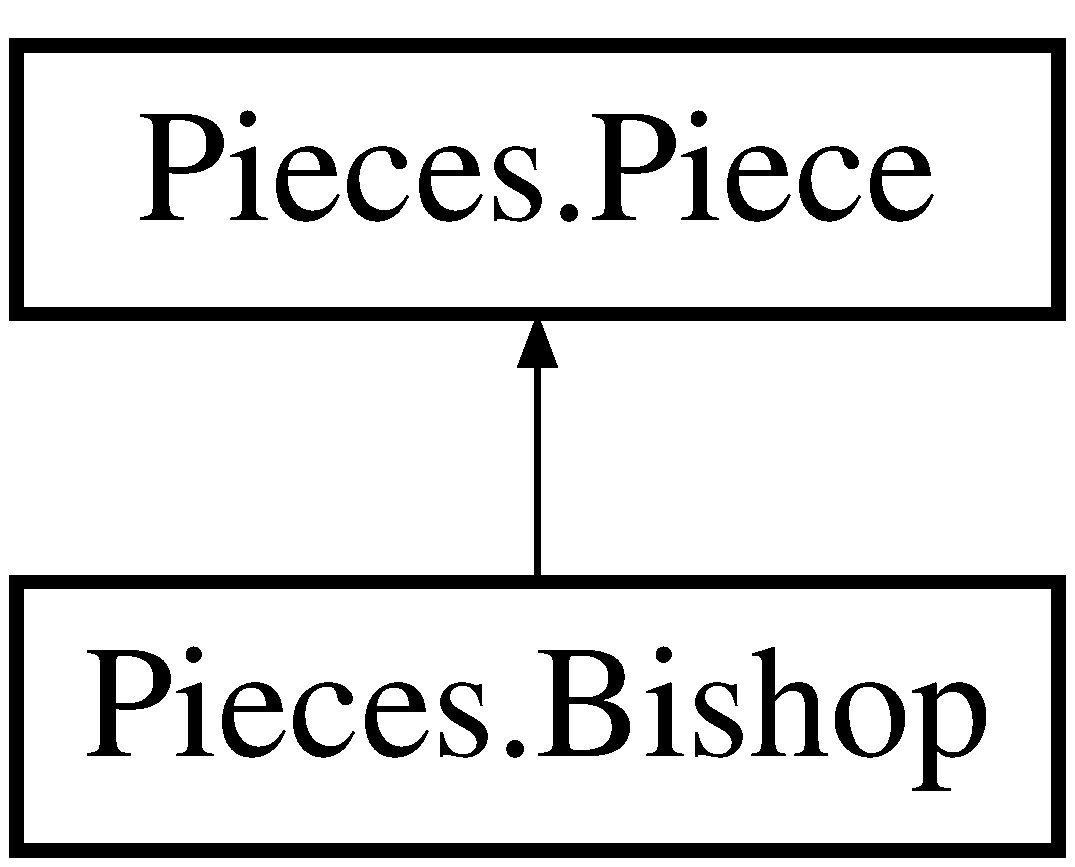
\includegraphics[height=2.000000cm]{classPieces_1_1Bishop}
\end{center}
\end{figure}
\subsection*{Public Member Functions}
\begin{DoxyCompactItemize}
\item 
\hyperlink{classPieces_1_1Bishop_a90daac09bc8f3b72059d8d8bb58a2114}{Bishop} (\hyperlink{classPieces_1_1Board}{Board} board, \hyperlink{classPieces_1_1Location}{Location} location, boolean owner)
\item 
boolean \hyperlink{classPieces_1_1Bishop_a0f854a40e1cf35efead6c52374356d17}{valid\-Move} (int des\-\_\-x, int des\-\_\-y)
\end{DoxyCompactItemize}


\subsection{Detailed Description}
Created by yutong on 9/7/16. 

\subsection{Constructor \& Destructor Documentation}
\hypertarget{classPieces_1_1Bishop_a90daac09bc8f3b72059d8d8bb58a2114}{\index{Pieces\-::\-Bishop@{Pieces\-::\-Bishop}!Bishop@{Bishop}}
\index{Bishop@{Bishop}!Pieces::Bishop@{Pieces\-::\-Bishop}}
\subsubsection[{Bishop}]{\setlength{\rightskip}{0pt plus 5cm}Pieces.\-Bishop.\-Bishop (
\begin{DoxyParamCaption}
\item[{{\bf Board}}]{board, }
\item[{{\bf Location}}]{location, }
\item[{boolean}]{owner}
\end{DoxyParamCaption}
)\hspace{0.3cm}{\ttfamily [inline]}}}\label{classPieces_1_1Bishop_a90daac09bc8f3b72059d8d8bb58a2114}
constructor for bishop 
\begin{DoxyParams}{Parameters}
{\em board} & game board \\
\hline
{\em location} & piece location \\
\hline
{\em owner} & piece owner \\
\hline
\end{DoxyParams}


\subsection{Member Function Documentation}
\hypertarget{classPieces_1_1Bishop_a0f854a40e1cf35efead6c52374356d17}{\index{Pieces\-::\-Bishop@{Pieces\-::\-Bishop}!valid\-Move@{valid\-Move}}
\index{valid\-Move@{valid\-Move}!Pieces::Bishop@{Pieces\-::\-Bishop}}
\subsubsection[{valid\-Move}]{\setlength{\rightskip}{0pt plus 5cm}boolean Pieces.\-Bishop.\-valid\-Move (
\begin{DoxyParamCaption}
\item[{int}]{des\-\_\-x, }
\item[{int}]{des\-\_\-y}
\end{DoxyParamCaption}
)\hspace{0.3cm}{\ttfamily [inline]}, {\ttfamily [virtual]}}}\label{classPieces_1_1Bishop_a0f854a40e1cf35efead6c52374356d17}

\begin{DoxyParams}{Parameters}
{\em des\-\_\-x} & coordinate x of destination tile \\
\hline
{\em des\-\_\-y} & coordinate y of destination tile \\
\hline
\end{DoxyParams}
\begin{DoxyReturn}{Returns}
return true if it's a valid bishop move and no piece is blocking it, false o/w 
\end{DoxyReturn}


Implements \hyperlink{classPieces_1_1Piece}{Pieces.\-Piece}.



The documentation for this class was generated from the following file\-:\begin{DoxyCompactItemize}
\item 
src/\-Pieces/Bishop.\-java\end{DoxyCompactItemize}

\hypertarget{classTests_1_1BishopTest}{\section{Tests.\-Bishop\-Test Class Reference}
\label{classTests_1_1BishopTest}\index{Tests.\-Bishop\-Test@{Tests.\-Bishop\-Test}}
}
\subsection*{Public Member Functions}
\begin{DoxyCompactItemize}
\item 
\hypertarget{classTests_1_1BishopTest_ae43c2bc5d02aa3a1a1338efd25081020}{void {\bfseries test} ()}\label{classTests_1_1BishopTest_ae43c2bc5d02aa3a1a1338efd25081020}

\item 
\hypertarget{classTests_1_1BishopTest_ac70b3913f45db662be354e2835c8922a}{void {\bfseries is\-Valid} ()}\label{classTests_1_1BishopTest_ac70b3913f45db662be354e2835c8922a}

\end{DoxyCompactItemize}


\subsection{Detailed Description}
Created by yutong on 9/7/16. 

The documentation for this class was generated from the following file\-:\begin{DoxyCompactItemize}
\item 
src/\-Tests/Bishop\-Test.\-java\end{DoxyCompactItemize}

\hypertarget{classPieces_1_1Board}{\section{Pieces.\-Board Class Reference}
\label{classPieces_1_1Board}\index{Pieces.\-Board@{Pieces.\-Board}}
}
\subsection*{Public Member Functions}
\begin{DoxyCompactItemize}
\item 
\hypertarget{classPieces_1_1Board_a5b88acf39af28ae35203fdc2726b5d30}{\hyperlink{classPieces_1_1Piece}{Piece}\mbox{[}$\,$\mbox{]}\mbox{[}$\,$\mbox{]} {\bfseries get\-Board} ()}\label{classPieces_1_1Board_a5b88acf39af28ae35203fdc2726b5d30}

\item 
\hypertarget{classPieces_1_1Board_a2417b574df42d2d2fe0bb30b2362829f}{\hyperlink{classPieces_1_1Piece}{Piece} {\bfseries get\-Piece} (int i, int j)}\label{classPieces_1_1Board_a2417b574df42d2d2fe0bb30b2362829f}

\item 
boolean \hyperlink{classPieces_1_1Board_aea9bbc7c7ba0a38264e2bccb53b57944}{can\-Move} (int i, int j, Object O)
\item 
void \hyperlink{classPieces_1_1Board_abf2357a58cfc3dc41a70538203185e85}{add\-Piece} (\hyperlink{classPieces_1_1Piece}{Piece} p, \hyperlink{classPieces_1_1Location}{Location} location)
\item 
void \hyperlink{classPieces_1_1Board_a7adb66ee30f16a87e8857d936de44610}{init\-Piece} (\hyperlink{classPieces_1_1Piece}{Piece} p)
\item 
void \hyperlink{classPieces_1_1Board_a01edc50a8996328e62a476a363c3901d}{remove\-Piece} (\hyperlink{classPieces_1_1Piece}{Piece} p)
\item 
void \hyperlink{classPieces_1_1Board_af5e7fe0f867051c7445abbec349600eb}{move\-Piece} (\hyperlink{classPieces_1_1Piece}{Piece} p, \hyperlink{classPieces_1_1Location}{Location} location)
\item 
\hyperlink{classPieces_1_1Location}{Location}\mbox{[}$\,$\mbox{]} \hyperlink{classPieces_1_1Board_a7e38dc282c0bdcc090e4a9ac3a632943}{get\-Path} (int cur\-\_\-x, int cur\-\_\-y, int des\-\_\-x, int des\-\_\-y)
\end{DoxyCompactItemize}


\subsection{Detailed Description}
Created by yutong on 9/7/16. 

\subsection{Member Function Documentation}
\hypertarget{classPieces_1_1Board_abf2357a58cfc3dc41a70538203185e85}{\index{Pieces\-::\-Board@{Pieces\-::\-Board}!add\-Piece@{add\-Piece}}
\index{add\-Piece@{add\-Piece}!Pieces::Board@{Pieces\-::\-Board}}
\subsubsection[{add\-Piece}]{\setlength{\rightskip}{0pt plus 5cm}void Pieces.\-Board.\-add\-Piece (
\begin{DoxyParamCaption}
\item[{{\bf Piece}}]{p, }
\item[{{\bf Location}}]{location}
\end{DoxyParamCaption}
)\hspace{0.3cm}{\ttfamily [inline]}}}\label{classPieces_1_1Board_abf2357a58cfc3dc41a70538203185e85}
add a piece to a location 
\begin{DoxyParams}{Parameters}
{\em p} & target piece p \\
\hline
{\em location} & destination location \\
\hline
\end{DoxyParams}
\hypertarget{classPieces_1_1Board_aea9bbc7c7ba0a38264e2bccb53b57944}{\index{Pieces\-::\-Board@{Pieces\-::\-Board}!can\-Move@{can\-Move}}
\index{can\-Move@{can\-Move}!Pieces::Board@{Pieces\-::\-Board}}
\subsubsection[{can\-Move}]{\setlength{\rightskip}{0pt plus 5cm}boolean Pieces.\-Board.\-can\-Move (
\begin{DoxyParamCaption}
\item[{int}]{i, }
\item[{int}]{j, }
\item[{Object}]{O}
\end{DoxyParamCaption}
)\hspace{0.3cm}{\ttfamily [inline]}}}\label{classPieces_1_1Board_aea9bbc7c7ba0a38264e2bccb53b57944}
move a piece to location (i,j) 
\begin{DoxyParams}{Parameters}
{\em i} & coordinate x of destination tile \\
\hline
{\em j} & coordinate y of destination tile \\
\hline
{\em O} & an arbitrary piece \\
\hline
\end{DoxyParams}
\begin{DoxyReturn}{Returns}
return true if it's a valid move, o/w return false 
\end{DoxyReturn}
\hypertarget{classPieces_1_1Board_a7e38dc282c0bdcc090e4a9ac3a632943}{\index{Pieces\-::\-Board@{Pieces\-::\-Board}!get\-Path@{get\-Path}}
\index{get\-Path@{get\-Path}!Pieces::Board@{Pieces\-::\-Board}}
\subsubsection[{get\-Path}]{\setlength{\rightskip}{0pt plus 5cm}{\bf Location} \mbox{[}$\,$\mbox{]} Pieces.\-Board.\-get\-Path (
\begin{DoxyParamCaption}
\item[{int}]{cur\-\_\-x, }
\item[{int}]{cur\-\_\-y, }
\item[{int}]{des\-\_\-x, }
\item[{int}]{des\-\_\-y}
\end{DoxyParamCaption}
)\hspace{0.3cm}{\ttfamily [inline]}}}\label{classPieces_1_1Board_a7e38dc282c0bdcc090e4a9ac3a632943}

\begin{DoxyParams}{Parameters}
{\em cur\-\_\-x} & piece that is currently under attack, coord x \\
\hline
{\em cur\-\_\-y} & piece that is currently under attack, coord y \\
\hline
{\em des\-\_\-x} & attacker, coord x \\
\hline
{\em des\-\_\-y} & attacker, coord y \\
\hline
\end{DoxyParams}
\begin{DoxyReturn}{Returns}
return an array of locations that forms the path from attacker to defender, including attackers location since attackers might be killed by other pieces. return null if it's an invalid path. 
\end{DoxyReturn}
\hypertarget{classPieces_1_1Board_a7adb66ee30f16a87e8857d936de44610}{\index{Pieces\-::\-Board@{Pieces\-::\-Board}!init\-Piece@{init\-Piece}}
\index{init\-Piece@{init\-Piece}!Pieces::Board@{Pieces\-::\-Board}}
\subsubsection[{init\-Piece}]{\setlength{\rightskip}{0pt plus 5cm}void Pieces.\-Board.\-init\-Piece (
\begin{DoxyParamCaption}
\item[{{\bf Piece}}]{p}
\end{DoxyParamCaption}
)\hspace{0.3cm}{\ttfamily [inline]}}}\label{classPieces_1_1Board_a7adb66ee30f16a87e8857d936de44610}
initialize a piece on the board 
\begin{DoxyParams}{Parameters}
{\em p} & target piece p \\
\hline
\end{DoxyParams}
\hypertarget{classPieces_1_1Board_af5e7fe0f867051c7445abbec349600eb}{\index{Pieces\-::\-Board@{Pieces\-::\-Board}!move\-Piece@{move\-Piece}}
\index{move\-Piece@{move\-Piece}!Pieces::Board@{Pieces\-::\-Board}}
\subsubsection[{move\-Piece}]{\setlength{\rightskip}{0pt plus 5cm}void Pieces.\-Board.\-move\-Piece (
\begin{DoxyParamCaption}
\item[{{\bf Piece}}]{p, }
\item[{{\bf Location}}]{location}
\end{DoxyParamCaption}
)\hspace{0.3cm}{\ttfamily [inline]}}}\label{classPieces_1_1Board_af5e7fe0f867051c7445abbec349600eb}
move a piece to the designated location 
\begin{DoxyParams}{Parameters}
{\em p} & piece p \\
\hline
{\em location} & destination location \\
\hline
\end{DoxyParams}
\hypertarget{classPieces_1_1Board_a01edc50a8996328e62a476a363c3901d}{\index{Pieces\-::\-Board@{Pieces\-::\-Board}!remove\-Piece@{remove\-Piece}}
\index{remove\-Piece@{remove\-Piece}!Pieces::Board@{Pieces\-::\-Board}}
\subsubsection[{remove\-Piece}]{\setlength{\rightskip}{0pt plus 5cm}void Pieces.\-Board.\-remove\-Piece (
\begin{DoxyParamCaption}
\item[{{\bf Piece}}]{p}
\end{DoxyParamCaption}
)\hspace{0.3cm}{\ttfamily [inline]}}}\label{classPieces_1_1Board_a01edc50a8996328e62a476a363c3901d}
remove a piece from the board 
\begin{DoxyParams}{Parameters}
{\em p} & target piece p \\
\hline
\end{DoxyParams}


The documentation for this class was generated from the following file\-:\begin{DoxyCompactItemize}
\item 
src/\-Pieces/Board.\-java\end{DoxyCompactItemize}

\hypertarget{classTests_1_1CheckmateTest}{\section{Tests.\-Checkmate\-Test Class Reference}
\label{classTests_1_1CheckmateTest}\index{Tests.\-Checkmate\-Test@{Tests.\-Checkmate\-Test}}
}
\subsection*{Public Member Functions}
\begin{DoxyCompactItemize}
\item 
\hypertarget{classTests_1_1CheckmateTest_ae95e3b938a1a132d72c5f542bbe52912}{void {\bfseries test} ()}\label{classTests_1_1CheckmateTest_ae95e3b938a1a132d72c5f542bbe52912}

\end{DoxyCompactItemize}


\subsection{Detailed Description}
Created by yutong on 9/8/16. 

The documentation for this class was generated from the following file\-:\begin{DoxyCompactItemize}
\item 
src/\-Tests/Checkmate\-Test.\-java\end{DoxyCompactItemize}

\hypertarget{classGUI_1_1ChessPiece}{\section{G\-U\-I.\-Chess\-Piece Class Reference}
\label{classGUI_1_1ChessPiece}\index{G\-U\-I.\-Chess\-Piece@{G\-U\-I.\-Chess\-Piece}}
}
\subsection*{Public Member Functions}
\begin{DoxyCompactItemize}
\item 
\hypertarget{classGUI_1_1ChessPiece_a405349b7705486d3ccecda990c80afce}{{\bfseries Chess\-Piece} (\hyperlink{classPieces_1_1Piece}{Piece} piece)}\label{classGUI_1_1ChessPiece_a405349b7705486d3ccecda990c80afce}

\item 
\hypertarget{classGUI_1_1ChessPiece_a4abc8a9a8082d4ea8147099477a34f7e}{\hyperlink{classPieces_1_1Location}{Location} {\bfseries get\-Location} ()}\label{classGUI_1_1ChessPiece_a4abc8a9a8082d4ea8147099477a34f7e}

\item 
Buffered\-Image \hyperlink{classGUI_1_1ChessPiece_ae7526af974247c7abebb011531484d72}{get\-Image} ()
\end{DoxyCompactItemize}


\subsection{Detailed Description}
Created by yutong on 9/14/16. 

\subsection{Member Function Documentation}
\hypertarget{classGUI_1_1ChessPiece_ae7526af974247c7abebb011531484d72}{\index{G\-U\-I\-::\-Chess\-Piece@{G\-U\-I\-::\-Chess\-Piece}!get\-Image@{get\-Image}}
\index{get\-Image@{get\-Image}!GUI::ChessPiece@{G\-U\-I\-::\-Chess\-Piece}}
\subsubsection[{get\-Image}]{\setlength{\rightskip}{0pt plus 5cm}Buffered\-Image G\-U\-I.\-Chess\-Piece.\-get\-Image (
\begin{DoxyParamCaption}
{}
\end{DoxyParamCaption}
)\hspace{0.3cm}{\ttfamily [inline]}}}\label{classGUI_1_1ChessPiece_ae7526af974247c7abebb011531484d72}
\begin{DoxyReturn}{Returns}
bufferedimage of a piece 
\end{DoxyReturn}


The documentation for this class was generated from the following file\-:\begin{DoxyCompactItemize}
\item 
src/\-G\-U\-I/Chess\-Piece.\-java\end{DoxyCompactItemize}

\hypertarget{classGUI_1_1Game}{\section{G\-U\-I.\-Game Class Reference}
\label{classGUI_1_1Game}\index{G\-U\-I.\-Game@{G\-U\-I.\-Game}}
}
\subsection*{Public Member Functions}
\begin{DoxyCompactItemize}
\item 
\hyperlink{classGUI_1_1Game_a97c23a5cb3fed78d68ef75d6d889b77a}{Game} ()
\end{DoxyCompactItemize}


\subsection{Detailed Description}
Created by yutong on 9/14/16. 

\subsection{Constructor \& Destructor Documentation}
\hypertarget{classGUI_1_1Game_a97c23a5cb3fed78d68ef75d6d889b77a}{\index{G\-U\-I\-::\-Game@{G\-U\-I\-::\-Game}!Game@{Game}}
\index{Game@{Game}!GUI::Game@{G\-U\-I\-::\-Game}}
\subsubsection[{Game}]{\setlength{\rightskip}{0pt plus 5cm}G\-U\-I.\-Game.\-Game (
\begin{DoxyParamCaption}
{}
\end{DoxyParamCaption}
)\hspace{0.3cm}{\ttfamily [inline]}}}\label{classGUI_1_1Game_a97c23a5cb3fed78d68ef75d6d889b77a}
constructor of the game 

The documentation for this class was generated from the following file\-:\begin{DoxyCompactItemize}
\item 
src/\-G\-U\-I/Game.\-java\end{DoxyCompactItemize}

\hypertarget{classPieces_1_1King}{\section{Pieces.\-King Class Reference}
\label{classPieces_1_1King}\index{Pieces.\-King@{Pieces.\-King}}
}
Inheritance diagram for Pieces.\-King\-:\begin{figure}[H]
\begin{center}
\leavevmode
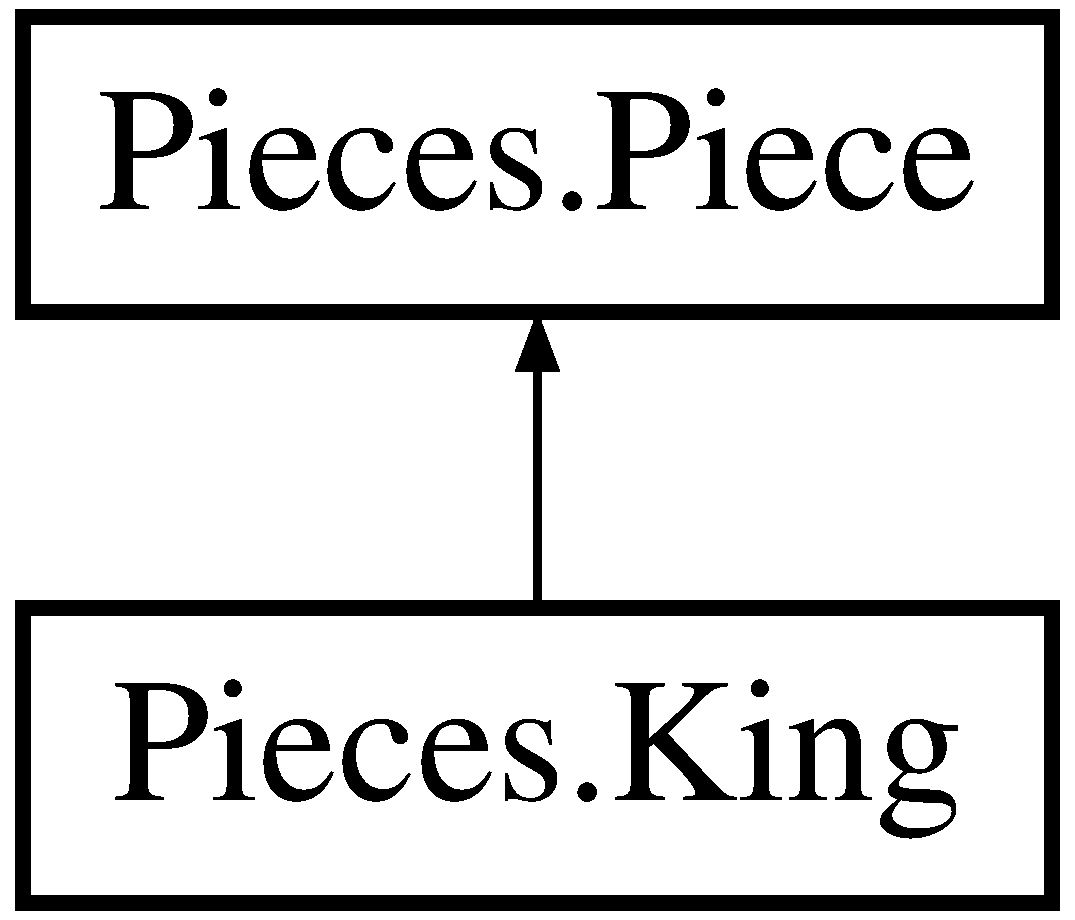
\includegraphics[height=2.000000cm]{classPieces_1_1King}
\end{center}
\end{figure}
\subsection*{Public Member Functions}
\begin{DoxyCompactItemize}
\item 
\hyperlink{classPieces_1_1King_a1df4d6e298eac55c704aff8e65d9fc48}{King} (\hyperlink{classPieces_1_1Board}{Board} board, \hyperlink{classPieces_1_1Location}{Location} location, boolean owner)
\item 
boolean \hyperlink{classPieces_1_1King_a0704fc0a6fba08b50db2aeed6734acc4}{valid\-Move} (int des\-\_\-x, int des\-\_\-y)
\end{DoxyCompactItemize}


\subsection{Detailed Description}
Created by yutong on 9/7/16. 

\subsection{Constructor \& Destructor Documentation}
\hypertarget{classPieces_1_1King_a1df4d6e298eac55c704aff8e65d9fc48}{\index{Pieces\-::\-King@{Pieces\-::\-King}!King@{King}}
\index{King@{King}!Pieces::King@{Pieces\-::\-King}}
\subsubsection[{King}]{\setlength{\rightskip}{0pt plus 5cm}Pieces.\-King.\-King (
\begin{DoxyParamCaption}
\item[{{\bf Board}}]{board, }
\item[{{\bf Location}}]{location, }
\item[{boolean}]{owner}
\end{DoxyParamCaption}
)\hspace{0.3cm}{\ttfamily [inline]}}}\label{classPieces_1_1King_a1df4d6e298eac55c704aff8e65d9fc48}
constructor for king 
\begin{DoxyParams}{Parameters}
{\em board} & game board \\
\hline
{\em location} & piece location \\
\hline
{\em owner} & piece owner \\
\hline
\end{DoxyParams}


\subsection{Member Function Documentation}
\hypertarget{classPieces_1_1King_a0704fc0a6fba08b50db2aeed6734acc4}{\index{Pieces\-::\-King@{Pieces\-::\-King}!valid\-Move@{valid\-Move}}
\index{valid\-Move@{valid\-Move}!Pieces::King@{Pieces\-::\-King}}
\subsubsection[{valid\-Move}]{\setlength{\rightskip}{0pt plus 5cm}boolean Pieces.\-King.\-valid\-Move (
\begin{DoxyParamCaption}
\item[{int}]{des\-\_\-x, }
\item[{int}]{des\-\_\-y}
\end{DoxyParamCaption}
)\hspace{0.3cm}{\ttfamily [inline]}, {\ttfamily [virtual]}}}\label{classPieces_1_1King_a0704fc0a6fba08b50db2aeed6734acc4}

\begin{DoxyParams}{Parameters}
{\em des\-\_\-x} & coordinate x of destination tile \\
\hline
{\em des\-\_\-y} & coordinate y of destination tile \\
\hline
\end{DoxyParams}
\begin{DoxyReturn}{Returns}
return true if it's a valid king move and no piece is blocking it, false o/w 
\end{DoxyReturn}


Implements \hyperlink{classPieces_1_1Piece}{Pieces.\-Piece}.



The documentation for this class was generated from the following file\-:\begin{DoxyCompactItemize}
\item 
src/\-Pieces/King.\-java\end{DoxyCompactItemize}

\hypertarget{classTests_1_1KingTest}{\section{Tests.\-King\-Test Class Reference}
\label{classTests_1_1KingTest}\index{Tests.\-King\-Test@{Tests.\-King\-Test}}
}
\subsection*{Public Member Functions}
\begin{DoxyCompactItemize}
\item 
\hypertarget{classTests_1_1KingTest_ae382fc23b711db05996165878caf85fb}{void {\bfseries test} ()}\label{classTests_1_1KingTest_ae382fc23b711db05996165878caf85fb}

\item 
\hypertarget{classTests_1_1KingTest_a4864b7967fdc6e7e0c74f72cc21efbff}{void {\bfseries is\-Valid} ()}\label{classTests_1_1KingTest_a4864b7967fdc6e7e0c74f72cc21efbff}

\end{DoxyCompactItemize}


\subsection{Detailed Description}
Created by yutong on 9/7/16. 

The documentation for this class was generated from the following file\-:\begin{DoxyCompactItemize}
\item 
src/\-Tests/King\-Test.\-java\end{DoxyCompactItemize}

\hypertarget{classPieces_1_1Knight}{\section{Pieces.\-Knight Class Reference}
\label{classPieces_1_1Knight}\index{Pieces.\-Knight@{Pieces.\-Knight}}
}
Inheritance diagram for Pieces.\-Knight\-:\begin{figure}[H]
\begin{center}
\leavevmode
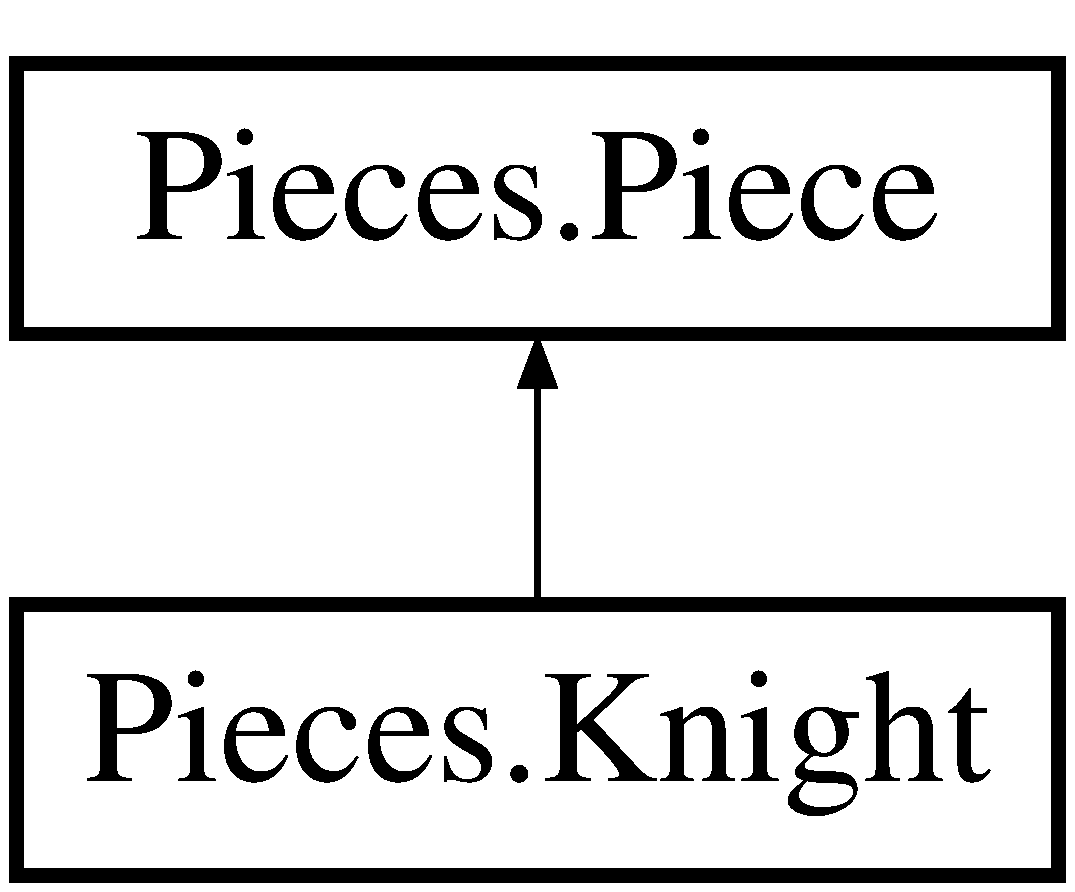
\includegraphics[height=2.000000cm]{classPieces_1_1Knight}
\end{center}
\end{figure}
\subsection*{Public Member Functions}
\begin{DoxyCompactItemize}
\item 
\hyperlink{classPieces_1_1Knight_a2556e996aa75ad0cd6e9e898c461e137}{Knight} (\hyperlink{classPieces_1_1Board}{Board} board, \hyperlink{classPieces_1_1Location}{Location} location, boolean owner)
\item 
boolean \hyperlink{classPieces_1_1Knight_a79b75fe95dcf838c0ff131bc3dc8db31}{valid\-Move} (int des\-\_\-x, int des\-\_\-y)
\end{DoxyCompactItemize}


\subsection{Detailed Description}
Created by yutong on 9/7/16. 

\subsection{Constructor \& Destructor Documentation}
\hypertarget{classPieces_1_1Knight_a2556e996aa75ad0cd6e9e898c461e137}{\index{Pieces\-::\-Knight@{Pieces\-::\-Knight}!Knight@{Knight}}
\index{Knight@{Knight}!Pieces::Knight@{Pieces\-::\-Knight}}
\subsubsection[{Knight}]{\setlength{\rightskip}{0pt plus 5cm}Pieces.\-Knight.\-Knight (
\begin{DoxyParamCaption}
\item[{{\bf Board}}]{board, }
\item[{{\bf Location}}]{location, }
\item[{boolean}]{owner}
\end{DoxyParamCaption}
)\hspace{0.3cm}{\ttfamily [inline]}}}\label{classPieces_1_1Knight_a2556e996aa75ad0cd6e9e898c461e137}
constructor for knight 
\begin{DoxyParams}{Parameters}
{\em board} & game board \\
\hline
{\em location} & piece location \\
\hline
{\em owner} & piece owner \\
\hline
\end{DoxyParams}


\subsection{Member Function Documentation}
\hypertarget{classPieces_1_1Knight_a79b75fe95dcf838c0ff131bc3dc8db31}{\index{Pieces\-::\-Knight@{Pieces\-::\-Knight}!valid\-Move@{valid\-Move}}
\index{valid\-Move@{valid\-Move}!Pieces::Knight@{Pieces\-::\-Knight}}
\subsubsection[{valid\-Move}]{\setlength{\rightskip}{0pt plus 5cm}boolean Pieces.\-Knight.\-valid\-Move (
\begin{DoxyParamCaption}
\item[{int}]{des\-\_\-x, }
\item[{int}]{des\-\_\-y}
\end{DoxyParamCaption}
)\hspace{0.3cm}{\ttfamily [inline]}, {\ttfamily [virtual]}}}\label{classPieces_1_1Knight_a79b75fe95dcf838c0ff131bc3dc8db31}

\begin{DoxyParams}{Parameters}
{\em des\-\_\-x} & coordinate x of destination tile \\
\hline
{\em des\-\_\-y} & coordinate y of destination tile \\
\hline
\end{DoxyParams}
\begin{DoxyReturn}{Returns}
return true if it's a valid knight move and no piece is blocking it, false o/w 
\end{DoxyReturn}


Implements \hyperlink{classPieces_1_1Piece}{Pieces.\-Piece}.



The documentation for this class was generated from the following file\-:\begin{DoxyCompactItemize}
\item 
src/\-Pieces/Knight.\-java\end{DoxyCompactItemize}

\hypertarget{classTests_1_1KnightTest}{\section{Tests.\-Knight\-Test Class Reference}
\label{classTests_1_1KnightTest}\index{Tests.\-Knight\-Test@{Tests.\-Knight\-Test}}
}
\subsection*{Public Member Functions}
\begin{DoxyCompactItemize}
\item 
\hypertarget{classTests_1_1KnightTest_a2172506c678c6551441630b290ff3856}{void {\bfseries test} ()}\label{classTests_1_1KnightTest_a2172506c678c6551441630b290ff3856}

\item 
\hypertarget{classTests_1_1KnightTest_ab5fc6398bec86b9761e731248092c7cd}{void {\bfseries is\-Valid} ()}\label{classTests_1_1KnightTest_ab5fc6398bec86b9761e731248092c7cd}

\end{DoxyCompactItemize}


\subsection{Detailed Description}
Created by yutong on 9/7/16. 

The documentation for this class was generated from the following file\-:\begin{DoxyCompactItemize}
\item 
src/\-Tests/Knight\-Test.\-java\end{DoxyCompactItemize}

\hypertarget{classPieces_1_1Location}{\section{Pieces.\-Location Class Reference}
\label{classPieces_1_1Location}\index{Pieces.\-Location@{Pieces.\-Location}}
}
\subsection*{Public Member Functions}
\begin{DoxyCompactItemize}
\item 
\hypertarget{classPieces_1_1Location_ad9d31ac2f03a07e98564d9318a576d7f}{{\bfseries Location} (int i, int j)}\label{classPieces_1_1Location_ad9d31ac2f03a07e98564d9318a576d7f}

\item 
\hypertarget{classPieces_1_1Location_aefc53c72a508b41d95f6f044df938161}{void {\bfseries set\-Location} (int i, int j)}\label{classPieces_1_1Location_aefc53c72a508b41d95f6f044df938161}

\item 
\hypertarget{classPieces_1_1Location_a5fa98ec99a45bcd20f7f3d3120ea3d4a}{int {\bfseries get\-Row} ()}\label{classPieces_1_1Location_a5fa98ec99a45bcd20f7f3d3120ea3d4a}

\item 
\hypertarget{classPieces_1_1Location_a3d8a453b994f35c7a14952f6dafede6c}{int {\bfseries get\-Col} ()}\label{classPieces_1_1Location_a3d8a453b994f35c7a14952f6dafede6c}

\end{DoxyCompactItemize}


\subsection{Detailed Description}
Created by yutong on 9/7/16. 

The documentation for this class was generated from the following file\-:\begin{DoxyCompactItemize}
\item 
src/\-Pieces/Location.\-java\end{DoxyCompactItemize}

\hypertarget{classPieces_1_1Logic}{\section{Pieces.\-Logic Class Reference}
\label{classPieces_1_1Logic}\index{Pieces.\-Logic@{Pieces.\-Logic}}
}
\subsection*{Public Member Functions}
\begin{DoxyCompactItemize}
\item 
\hyperlink{classPieces_1_1Piece}{Piece} \hyperlink{classPieces_1_1Logic_a8b2c1f370c82d9639758c409ea8d9d79}{get\-Piece} (int i, int j)
\item 
\hyperlink{classPieces_1_1Piece}{Piece} \hyperlink{classPieces_1_1Logic_ad83f352abf092e2740ab495d65a97ae9}{get\-King} (boolean owner)
\item 
\hyperlink{classPieces_1_1Piece}{Piece} \hyperlink{classPieces_1_1Logic_aec1ccc44beb7de53fd9077469feff9e8}{checked\-By\-Knight} (\hyperlink{classPieces_1_1Piece}{Piece} p)
\item 
\hyperlink{classPieces_1_1Piece}{Piece} \hyperlink{classPieces_1_1Logic_af1d641f37da06c3e45b5a6bee9a6525b}{checked\-Diagonal} (\hyperlink{classPieces_1_1Piece}{Piece} p)
\item 
\hyperlink{classPieces_1_1Piece}{Piece} \hyperlink{classPieces_1_1Logic_ac0bb52cd90a0dd7cacc10521eb2e57f8}{checked\-In\-Line} (\hyperlink{classPieces_1_1Piece}{Piece} p)
\item 
boolean \hyperlink{classPieces_1_1Logic_aaf2761d9be4c7aba979922d5919bea28}{is\-Checked} (\hyperlink{classPieces_1_1Piece}{Piece} p)
\item 
boolean \hyperlink{classPieces_1_1Logic_aaeeb3da7c87dc40646df2b3f1b4bc50e}{no\-Moves} (\hyperlink{classPieces_1_1Piece}{Piece} p)
\item 
boolean \hyperlink{classPieces_1_1Logic_a876ca4b44bc7042fd633f1545e46013a}{is\-Check\-Mate} (\hyperlink{classPieces_1_1Piece}{Piece} p)
\item 
boolean \hyperlink{classPieces_1_1Logic_a9d339891130cff2940891cdf85a0f248}{is\-Stale\-Mate} (\hyperlink{classPieces_1_1Piece}{Piece} p)
\end{DoxyCompactItemize}


\subsection{Detailed Description}
Created by yutong on 9/8/16. 

\subsection{Member Function Documentation}
\hypertarget{classPieces_1_1Logic_aec1ccc44beb7de53fd9077469feff9e8}{\index{Pieces\-::\-Logic@{Pieces\-::\-Logic}!checked\-By\-Knight@{checked\-By\-Knight}}
\index{checked\-By\-Knight@{checked\-By\-Knight}!Pieces::Logic@{Pieces\-::\-Logic}}
\subsubsection[{checked\-By\-Knight}]{\setlength{\rightskip}{0pt plus 5cm}{\bf Piece} Pieces.\-Logic.\-checked\-By\-Knight (
\begin{DoxyParamCaption}
\item[{{\bf Piece}}]{p}
\end{DoxyParamCaption}
)\hspace{0.3cm}{\ttfamily [inline]}}}\label{classPieces_1_1Logic_aec1ccc44beb7de53fd9077469feff9e8}

\begin{DoxyParams}{Parameters}
{\em p} & king \\
\hline
\end{DoxyParams}
\begin{DoxyReturn}{Returns}
return the knight that's checking the king, null o/w 
\end{DoxyReturn}
\hypertarget{classPieces_1_1Logic_af1d641f37da06c3e45b5a6bee9a6525b}{\index{Pieces\-::\-Logic@{Pieces\-::\-Logic}!checked\-Diagonal@{checked\-Diagonal}}
\index{checked\-Diagonal@{checked\-Diagonal}!Pieces::Logic@{Pieces\-::\-Logic}}
\subsubsection[{checked\-Diagonal}]{\setlength{\rightskip}{0pt plus 5cm}{\bf Piece} Pieces.\-Logic.\-checked\-Diagonal (
\begin{DoxyParamCaption}
\item[{{\bf Piece}}]{p}
\end{DoxyParamCaption}
)\hspace{0.3cm}{\ttfamily [inline]}}}\label{classPieces_1_1Logic_af1d641f37da06c3e45b5a6bee9a6525b}

\begin{DoxyParams}{Parameters}
{\em p} & king \\
\hline
\end{DoxyParams}
\begin{DoxyReturn}{Returns}
return the piece that's checking the king diagonally, null o/w 
\end{DoxyReturn}
\hypertarget{classPieces_1_1Logic_ac0bb52cd90a0dd7cacc10521eb2e57f8}{\index{Pieces\-::\-Logic@{Pieces\-::\-Logic}!checked\-In\-Line@{checked\-In\-Line}}
\index{checked\-In\-Line@{checked\-In\-Line}!Pieces::Logic@{Pieces\-::\-Logic}}
\subsubsection[{checked\-In\-Line}]{\setlength{\rightskip}{0pt plus 5cm}{\bf Piece} Pieces.\-Logic.\-checked\-In\-Line (
\begin{DoxyParamCaption}
\item[{{\bf Piece}}]{p}
\end{DoxyParamCaption}
)\hspace{0.3cm}{\ttfamily [inline]}}}\label{classPieces_1_1Logic_ac0bb52cd90a0dd7cacc10521eb2e57f8}

\begin{DoxyParams}{Parameters}
{\em p} & king \\
\hline
\end{DoxyParams}
\begin{DoxyReturn}{Returns}
return the piece that's checking the king vertically and horizontally, null o/w 
\end{DoxyReturn}
\hypertarget{classPieces_1_1Logic_ad83f352abf092e2740ab495d65a97ae9}{\index{Pieces\-::\-Logic@{Pieces\-::\-Logic}!get\-King@{get\-King}}
\index{get\-King@{get\-King}!Pieces::Logic@{Pieces\-::\-Logic}}
\subsubsection[{get\-King}]{\setlength{\rightskip}{0pt plus 5cm}{\bf Piece} Pieces.\-Logic.\-get\-King (
\begin{DoxyParamCaption}
\item[{boolean}]{owner}
\end{DoxyParamCaption}
)\hspace{0.3cm}{\ttfamily [inline]}}}\label{classPieces_1_1Logic_ad83f352abf092e2740ab495d65a97ae9}

\begin{DoxyParams}{Parameters}
{\em owner} & ownership of a piece \\
\hline
\end{DoxyParams}
\begin{DoxyReturn}{Returns}
the king of one player 
\end{DoxyReturn}
\hypertarget{classPieces_1_1Logic_a8b2c1f370c82d9639758c409ea8d9d79}{\index{Pieces\-::\-Logic@{Pieces\-::\-Logic}!get\-Piece@{get\-Piece}}
\index{get\-Piece@{get\-Piece}!Pieces::Logic@{Pieces\-::\-Logic}}
\subsubsection[{get\-Piece}]{\setlength{\rightskip}{0pt plus 5cm}{\bf Piece} Pieces.\-Logic.\-get\-Piece (
\begin{DoxyParamCaption}
\item[{int}]{i, }
\item[{int}]{j}
\end{DoxyParamCaption}
)\hspace{0.3cm}{\ttfamily [inline]}}}\label{classPieces_1_1Logic_a8b2c1f370c82d9639758c409ea8d9d79}

\begin{DoxyParams}{Parameters}
{\em i} & coordinate x of destination tile \\
\hline
{\em j} & coordinate y of destination tile \\
\hline
\end{DoxyParams}
\begin{DoxyReturn}{Returns}
return the piece on the destination tile 
\end{DoxyReturn}
\hypertarget{classPieces_1_1Logic_aaf2761d9be4c7aba979922d5919bea28}{\index{Pieces\-::\-Logic@{Pieces\-::\-Logic}!is\-Checked@{is\-Checked}}
\index{is\-Checked@{is\-Checked}!Pieces::Logic@{Pieces\-::\-Logic}}
\subsubsection[{is\-Checked}]{\setlength{\rightskip}{0pt plus 5cm}boolean Pieces.\-Logic.\-is\-Checked (
\begin{DoxyParamCaption}
\item[{{\bf Piece}}]{p}
\end{DoxyParamCaption}
)\hspace{0.3cm}{\ttfamily [inline]}}}\label{classPieces_1_1Logic_aaf2761d9be4c7aba979922d5919bea28}

\begin{DoxyParams}{Parameters}
{\em p} & king \\
\hline
\end{DoxyParams}
\begin{DoxyReturn}{Returns}
return true if the king is checked, false o/w 
\end{DoxyReturn}
\hypertarget{classPieces_1_1Logic_a876ca4b44bc7042fd633f1545e46013a}{\index{Pieces\-::\-Logic@{Pieces\-::\-Logic}!is\-Check\-Mate@{is\-Check\-Mate}}
\index{is\-Check\-Mate@{is\-Check\-Mate}!Pieces::Logic@{Pieces\-::\-Logic}}
\subsubsection[{is\-Check\-Mate}]{\setlength{\rightskip}{0pt plus 5cm}boolean Pieces.\-Logic.\-is\-Check\-Mate (
\begin{DoxyParamCaption}
\item[{{\bf Piece}}]{p}
\end{DoxyParamCaption}
)\hspace{0.3cm}{\ttfamily [inline]}}}\label{classPieces_1_1Logic_a876ca4b44bc7042fd633f1545e46013a}

\begin{DoxyParams}{Parameters}
{\em p} & king \\
\hline
\end{DoxyParams}
\begin{DoxyReturn}{Returns}
return true if the game is in checkmate, false o/w 
\end{DoxyReturn}
\hypertarget{classPieces_1_1Logic_a9d339891130cff2940891cdf85a0f248}{\index{Pieces\-::\-Logic@{Pieces\-::\-Logic}!is\-Stale\-Mate@{is\-Stale\-Mate}}
\index{is\-Stale\-Mate@{is\-Stale\-Mate}!Pieces::Logic@{Pieces\-::\-Logic}}
\subsubsection[{is\-Stale\-Mate}]{\setlength{\rightskip}{0pt plus 5cm}boolean Pieces.\-Logic.\-is\-Stale\-Mate (
\begin{DoxyParamCaption}
\item[{{\bf Piece}}]{p}
\end{DoxyParamCaption}
)\hspace{0.3cm}{\ttfamily [inline]}}}\label{classPieces_1_1Logic_a9d339891130cff2940891cdf85a0f248}

\begin{DoxyParams}{Parameters}
{\em p} & king \\
\hline
\end{DoxyParams}
\begin{DoxyReturn}{Returns}
return true if the game is stalemate, false o/w 
\end{DoxyReturn}
\hypertarget{classPieces_1_1Logic_aaeeb3da7c87dc40646df2b3f1b4bc50e}{\index{Pieces\-::\-Logic@{Pieces\-::\-Logic}!no\-Moves@{no\-Moves}}
\index{no\-Moves@{no\-Moves}!Pieces::Logic@{Pieces\-::\-Logic}}
\subsubsection[{no\-Moves}]{\setlength{\rightskip}{0pt plus 5cm}boolean Pieces.\-Logic.\-no\-Moves (
\begin{DoxyParamCaption}
\item[{{\bf Piece}}]{p}
\end{DoxyParamCaption}
)\hspace{0.3cm}{\ttfamily [inline]}}}\label{classPieces_1_1Logic_aaeeb3da7c87dc40646df2b3f1b4bc50e}

\begin{DoxyParams}{Parameters}
{\em p} & king \\
\hline
\end{DoxyParams}
\begin{DoxyReturn}{Returns}
return true if the king has no legal move, false o/w 
\end{DoxyReturn}


The documentation for this class was generated from the following file\-:\begin{DoxyCompactItemize}
\item 
src/\-Pieces/Logic.\-java\end{DoxyCompactItemize}

\hypertarget{classMain}{\section{Main Class Reference}
\label{classMain}\index{Main@{Main}}
}
\subsection*{Static Public Member Functions}
\begin{DoxyCompactItemize}
\item 
\hypertarget{classMain_ac4044c12d5a6392e6cbe6b60dd70d894}{static void {\bfseries main} (String\mbox{[}$\,$\mbox{]}args)}\label{classMain_ac4044c12d5a6392e6cbe6b60dd70d894}

\end{DoxyCompactItemize}


\subsection{Detailed Description}
Created by yutong on 9/14/16. 

The documentation for this class was generated from the following file\-:\begin{DoxyCompactItemize}
\item 
src/Main.\-java\end{DoxyCompactItemize}

\hypertarget{classPieces_1_1Pawn}{\section{Pieces.\-Pawn Class Reference}
\label{classPieces_1_1Pawn}\index{Pieces.\-Pawn@{Pieces.\-Pawn}}
}
Inheritance diagram for Pieces.\-Pawn\-:\begin{figure}[H]
\begin{center}
\leavevmode
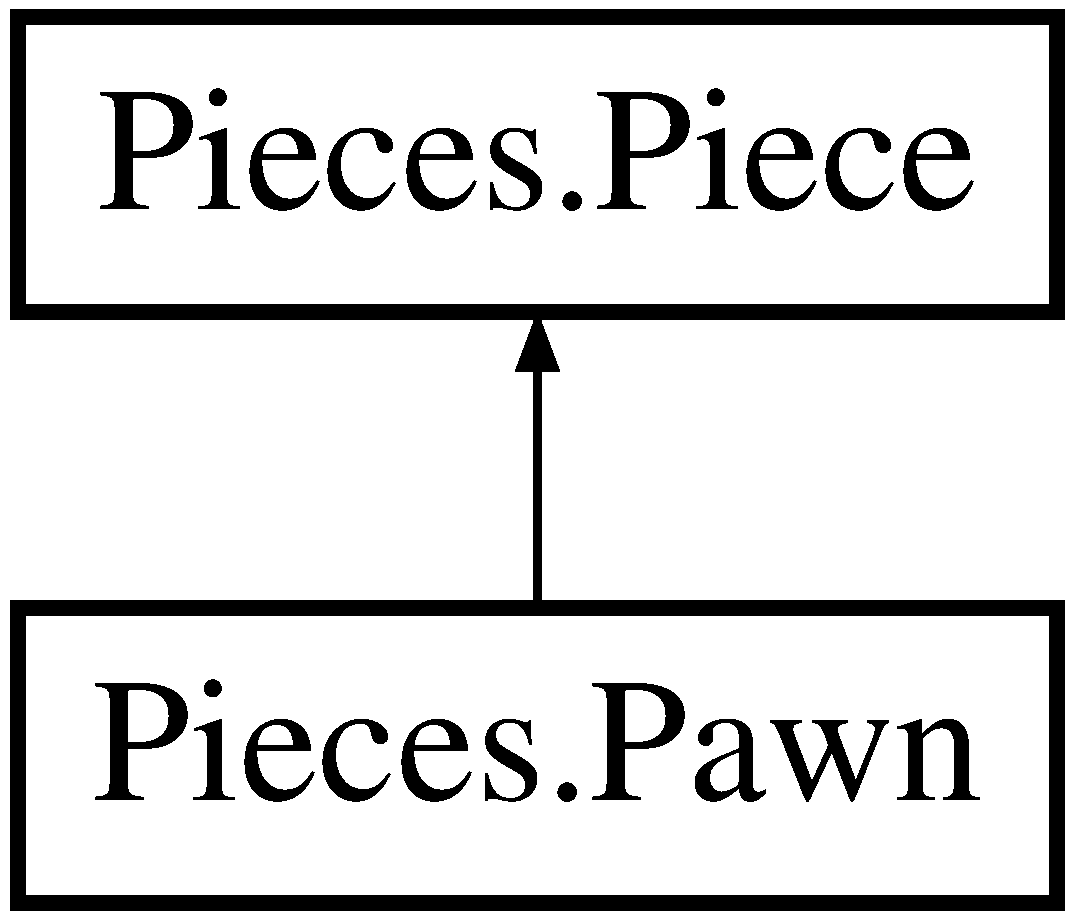
\includegraphics[height=2.000000cm]{classPieces_1_1Pawn}
\end{center}
\end{figure}
\subsection*{Public Member Functions}
\begin{DoxyCompactItemize}
\item 
boolean \hyperlink{classPieces_1_1Pawn_a80400d0f5bfade69ebcd06ccbd339835}{is\-First} ()
\item 
\hyperlink{classPieces_1_1Pawn_a4b162dc7bf4688bc79a5337110358e01}{Pawn} (\hyperlink{classPieces_1_1Board}{Board} board, \hyperlink{classPieces_1_1Location}{Location} location, boolean owner)
\item 
boolean \hyperlink{classPieces_1_1Pawn_a8fc4c6055b94785d65f0bf092ff3094a}{valid\-Move} (int des\-\_\-x, int des\-\_\-y)
\end{DoxyCompactItemize}


\subsection{Detailed Description}
Created by yutong on 9/4/16. 

\subsection{Constructor \& Destructor Documentation}
\hypertarget{classPieces_1_1Pawn_a4b162dc7bf4688bc79a5337110358e01}{\index{Pieces\-::\-Pawn@{Pieces\-::\-Pawn}!Pawn@{Pawn}}
\index{Pawn@{Pawn}!Pieces::Pawn@{Pieces\-::\-Pawn}}
\subsubsection[{Pawn}]{\setlength{\rightskip}{0pt plus 5cm}Pieces.\-Pawn.\-Pawn (
\begin{DoxyParamCaption}
\item[{{\bf Board}}]{board, }
\item[{{\bf Location}}]{location, }
\item[{boolean}]{owner}
\end{DoxyParamCaption}
)\hspace{0.3cm}{\ttfamily [inline]}}}\label{classPieces_1_1Pawn_a4b162dc7bf4688bc79a5337110358e01}
constructor for pawn 
\begin{DoxyParams}{Parameters}
{\em board} & game board \\
\hline
{\em location} & piece location \\
\hline
{\em owner} & piece owner \\
\hline
\end{DoxyParams}


\subsection{Member Function Documentation}
\hypertarget{classPieces_1_1Pawn_a80400d0f5bfade69ebcd06ccbd339835}{\index{Pieces\-::\-Pawn@{Pieces\-::\-Pawn}!is\-First@{is\-First}}
\index{is\-First@{is\-First}!Pieces::Pawn@{Pieces\-::\-Pawn}}
\subsubsection[{is\-First}]{\setlength{\rightskip}{0pt plus 5cm}boolean Pieces.\-Pawn.\-is\-First (
\begin{DoxyParamCaption}
{}
\end{DoxyParamCaption}
)\hspace{0.3cm}{\ttfamily [inline]}}}\label{classPieces_1_1Pawn_a80400d0f5bfade69ebcd06ccbd339835}
\begin{DoxyReturn}{Returns}
true if it's the first move of a pawn, false o/w 
\end{DoxyReturn}
\hypertarget{classPieces_1_1Pawn_a8fc4c6055b94785d65f0bf092ff3094a}{\index{Pieces\-::\-Pawn@{Pieces\-::\-Pawn}!valid\-Move@{valid\-Move}}
\index{valid\-Move@{valid\-Move}!Pieces::Pawn@{Pieces\-::\-Pawn}}
\subsubsection[{valid\-Move}]{\setlength{\rightskip}{0pt plus 5cm}boolean Pieces.\-Pawn.\-valid\-Move (
\begin{DoxyParamCaption}
\item[{int}]{des\-\_\-x, }
\item[{int}]{des\-\_\-y}
\end{DoxyParamCaption}
)\hspace{0.3cm}{\ttfamily [inline]}, {\ttfamily [virtual]}}}\label{classPieces_1_1Pawn_a8fc4c6055b94785d65f0bf092ff3094a}

\begin{DoxyParams}{Parameters}
{\em des\-\_\-x} & coord x of destination tile \\
\hline
{\em des\-\_\-y} & coord y of destination tile \\
\hline
\end{DoxyParams}
\begin{DoxyReturn}{Returns}
true if it's a valid pawn move, false o/w 
\end{DoxyReturn}


Implements \hyperlink{classPieces_1_1Piece}{Pieces.\-Piece}.



The documentation for this class was generated from the following file\-:\begin{DoxyCompactItemize}
\item 
src/\-Pieces/Pawn.\-java\end{DoxyCompactItemize}

\hypertarget{classTests_1_1PawnTest}{\section{Tests.\-Pawn\-Test Class Reference}
\label{classTests_1_1PawnTest}\index{Tests.\-Pawn\-Test@{Tests.\-Pawn\-Test}}
}
\subsection*{Public Member Functions}
\begin{DoxyCompactItemize}
\item 
\hypertarget{classTests_1_1PawnTest_a545e4a8a8bbaa7fd6dc1f7248b7f9274}{void {\bfseries test} ()}\label{classTests_1_1PawnTest_a545e4a8a8bbaa7fd6dc1f7248b7f9274}

\item 
\hypertarget{classTests_1_1PawnTest_a58495055dc7b2cc8078a285cd76f50a4}{void {\bfseries is\-Valid} ()}\label{classTests_1_1PawnTest_a58495055dc7b2cc8078a285cd76f50a4}

\end{DoxyCompactItemize}


\subsection{Detailed Description}
Created by yutong on 9/7/16. 

The documentation for this class was generated from the following file\-:\begin{DoxyCompactItemize}
\item 
src/\-Tests/Pawn\-Test.\-java\end{DoxyCompactItemize}

\hypertarget{classPieces_1_1Piece}{\section{Pieces.\-Piece Class Reference}
\label{classPieces_1_1Piece}\index{Pieces.\-Piece@{Pieces.\-Piece}}
}
Inheritance diagram for Pieces.\-Piece\-:\begin{figure}[H]
\begin{center}
\leavevmode
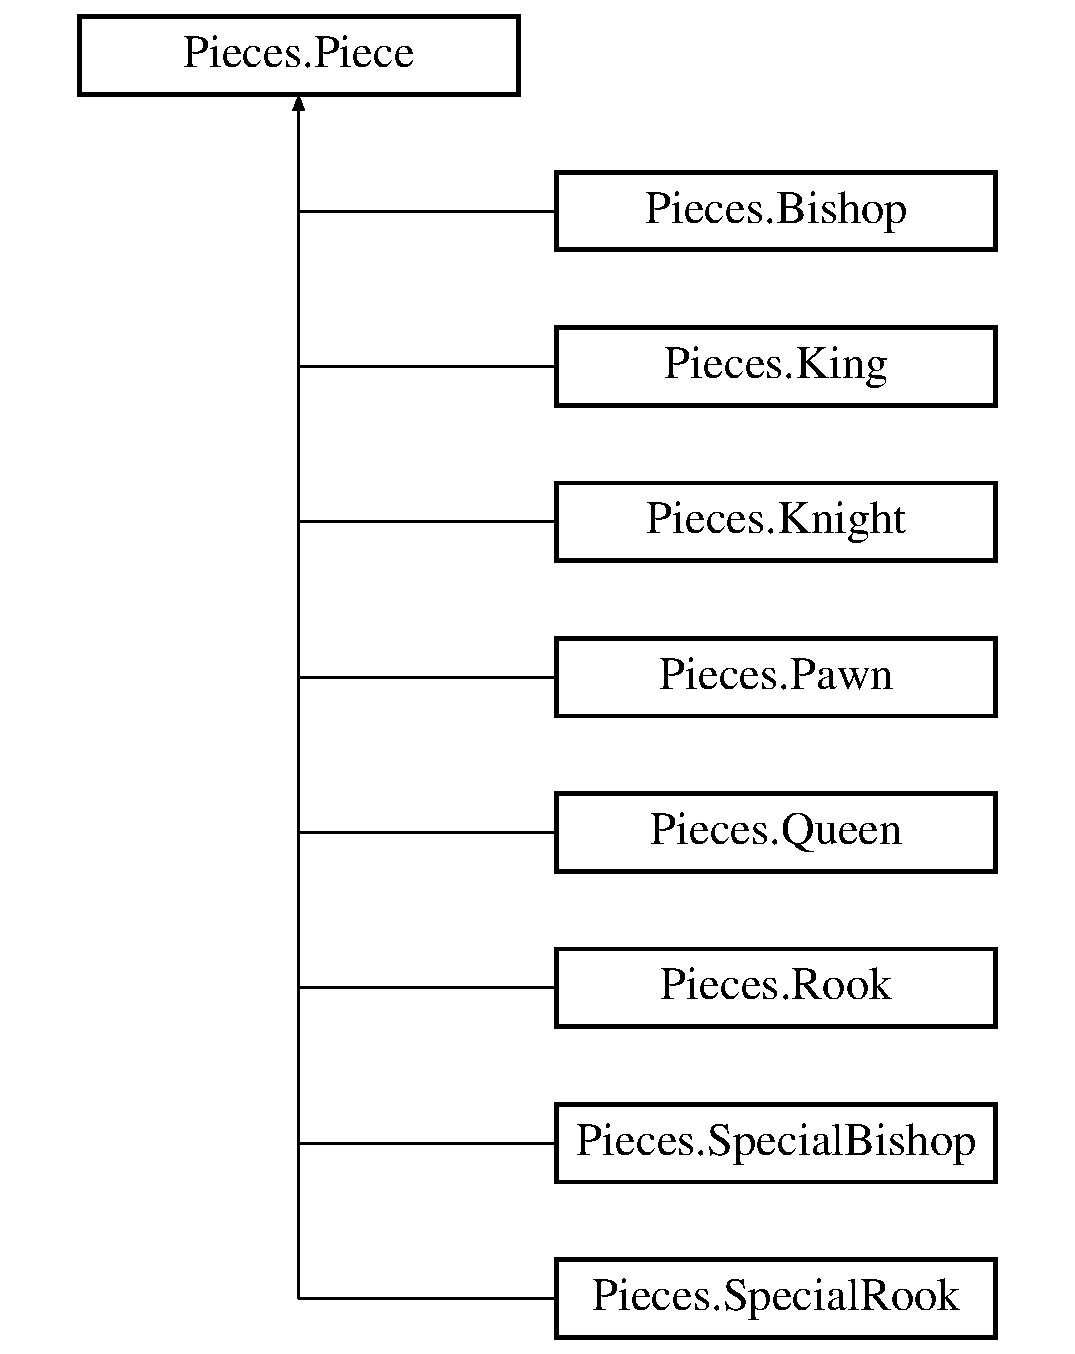
\includegraphics[height=9.000000cm]{classPieces_1_1Piece}
\end{center}
\end{figure}
\subsection*{Public Member Functions}
\begin{DoxyCompactItemize}
\item 
\hyperlink{classPieces_1_1Piece_a970bf8c665edd3574fadab1304798129}{Piece} (\hyperlink{classPieces_1_1Board}{Board} board, \hyperlink{classPieces_1_1Location}{Location} location, boolean owner)
\item 
\hypertarget{classPieces_1_1Piece_a01c050ca609d43e205923037a786823a}{abstract boolean {\bfseries valid\-Move} (int des\-\_\-x, int des\-\_\-y)}\label{classPieces_1_1Piece_a01c050ca609d43e205923037a786823a}

\item 
\hypertarget{classPieces_1_1Piece_a1163b80f94aeae277f557cdb34d23d39}{\hyperlink{classPieces_1_1Board}{Board} {\bfseries get\-Board} ()}\label{classPieces_1_1Piece_a1163b80f94aeae277f557cdb34d23d39}

\item 
\hypertarget{classPieces_1_1Piece_a402d4d6c7df72cd68415a25f2c1602e7}{\hyperlink{classPieces_1_1Location}{Location} {\bfseries get\-Location} ()}\label{classPieces_1_1Piece_a402d4d6c7df72cd68415a25f2c1602e7}

\item 
\hypertarget{classPieces_1_1Piece_ad18e2238bb732ffe521092b0dc8d12de}{boolean {\bfseries get\-Owner} ()}\label{classPieces_1_1Piece_ad18e2238bb732ffe521092b0dc8d12de}

\item 
\hypertarget{classPieces_1_1Piece_ab137d8249f1a4eb44acc4cad0826f75b}{void {\bfseries set\-Location} (\hyperlink{classPieces_1_1Location}{Location} location)}\label{classPieces_1_1Piece_ab137d8249f1a4eb44acc4cad0826f75b}

\item 
boolean \hyperlink{classPieces_1_1Piece_a5e66d12aa0a6be14976d0d6b19d4691b}{check\-Diagonally} (int cur\-\_\-x, int cur\-\_\-y, int des\-\_\-x, int des\-\_\-y)
\item 
boolean \hyperlink{classPieces_1_1Piece_a280fcf87182fd90bc66c8ee34a8107e6}{check\-In\-Line} (int cur\-\_\-x, int cur\-\_\-y, int des\-\_\-x, int des\-\_\-y)
\item 
boolean \hyperlink{classPieces_1_1Piece_af5d4a48732d86232e327c23d0b1fe1dc}{equals} (\hyperlink{classPieces_1_1Piece}{Piece} other)
\item 
boolean \hyperlink{classPieces_1_1Piece_a6f703962dfae61cd6d33c3abf36c43a1}{out\-Of\-Boundary} (int des\-\_\-x, int des\-\_\-y)
\item 
boolean \hyperlink{classPieces_1_1Piece_a61a09c26c02518e4cbb6da1389cb73d8}{didntmove} (int cur\-\_\-x, int cur\-\_\-y, int des\-\_\-x, int des\-\_\-y)
\end{DoxyCompactItemize}


\subsection{Detailed Description}
Created by yutong on 9/4/16. 

\subsection{Constructor \& Destructor Documentation}
\hypertarget{classPieces_1_1Piece_a970bf8c665edd3574fadab1304798129}{\index{Pieces\-::\-Piece@{Pieces\-::\-Piece}!Piece@{Piece}}
\index{Piece@{Piece}!Pieces::Piece@{Pieces\-::\-Piece}}
\subsubsection[{Piece}]{\setlength{\rightskip}{0pt plus 5cm}Pieces.\-Piece.\-Piece (
\begin{DoxyParamCaption}
\item[{{\bf Board}}]{board, }
\item[{{\bf Location}}]{location, }
\item[{boolean}]{owner}
\end{DoxyParamCaption}
)\hspace{0.3cm}{\ttfamily [inline]}}}\label{classPieces_1_1Piece_a970bf8c665edd3574fadab1304798129}
constructor for piece 
\begin{DoxyParams}{Parameters}
{\em board} & game board \\
\hline
{\em location} & piece location \\
\hline
{\em owner} & piece owner \\
\hline
\end{DoxyParams}


\subsection{Member Function Documentation}
\hypertarget{classPieces_1_1Piece_a5e66d12aa0a6be14976d0d6b19d4691b}{\index{Pieces\-::\-Piece@{Pieces\-::\-Piece}!check\-Diagonally@{check\-Diagonally}}
\index{check\-Diagonally@{check\-Diagonally}!Pieces::Piece@{Pieces\-::\-Piece}}
\subsubsection[{check\-Diagonally}]{\setlength{\rightskip}{0pt plus 5cm}boolean Pieces.\-Piece.\-check\-Diagonally (
\begin{DoxyParamCaption}
\item[{int}]{cur\-\_\-x, }
\item[{int}]{cur\-\_\-y, }
\item[{int}]{des\-\_\-x, }
\item[{int}]{des\-\_\-y}
\end{DoxyParamCaption}
)\hspace{0.3cm}{\ttfamily [inline]}}}\label{classPieces_1_1Piece_a5e66d12aa0a6be14976d0d6b19d4691b}

\begin{DoxyParams}{Parameters}
{\em cur\-\_\-x} & coordinate x of starting tile \\
\hline
{\em cur\-\_\-y} & coordinate y of starting tile \\
\hline
{\em des\-\_\-x} & coordinate x of destination tile \\
\hline
{\em des\-\_\-y} & coordinate y of destination tile \\
\hline
\end{DoxyParams}
\begin{DoxyReturn}{Returns}
Check path diagonally, True if the route is blocked, False o/w 
\end{DoxyReturn}
\hypertarget{classPieces_1_1Piece_a280fcf87182fd90bc66c8ee34a8107e6}{\index{Pieces\-::\-Piece@{Pieces\-::\-Piece}!check\-In\-Line@{check\-In\-Line}}
\index{check\-In\-Line@{check\-In\-Line}!Pieces::Piece@{Pieces\-::\-Piece}}
\subsubsection[{check\-In\-Line}]{\setlength{\rightskip}{0pt plus 5cm}boolean Pieces.\-Piece.\-check\-In\-Line (
\begin{DoxyParamCaption}
\item[{int}]{cur\-\_\-x, }
\item[{int}]{cur\-\_\-y, }
\item[{int}]{des\-\_\-x, }
\item[{int}]{des\-\_\-y}
\end{DoxyParamCaption}
)\hspace{0.3cm}{\ttfamily [inline]}}}\label{classPieces_1_1Piece_a280fcf87182fd90bc66c8ee34a8107e6}

\begin{DoxyParams}{Parameters}
{\em cur\-\_\-x} & coordinate x of starting tile \\
\hline
{\em cur\-\_\-y} & coordinate y of starting tile \\
\hline
{\em des\-\_\-x} & coordinate x of destination tile \\
\hline
{\em des\-\_\-y} & coordinate y of destination tile \\
\hline
\end{DoxyParams}
\begin{DoxyReturn}{Returns}
Check path horizontally and vertically, True if the route is blocked, False o/w 
\end{DoxyReturn}
\hypertarget{classPieces_1_1Piece_a61a09c26c02518e4cbb6da1389cb73d8}{\index{Pieces\-::\-Piece@{Pieces\-::\-Piece}!didntmove@{didntmove}}
\index{didntmove@{didntmove}!Pieces::Piece@{Pieces\-::\-Piece}}
\subsubsection[{didntmove}]{\setlength{\rightskip}{0pt plus 5cm}boolean Pieces.\-Piece.\-didntmove (
\begin{DoxyParamCaption}
\item[{int}]{cur\-\_\-x, }
\item[{int}]{cur\-\_\-y, }
\item[{int}]{des\-\_\-x, }
\item[{int}]{des\-\_\-y}
\end{DoxyParamCaption}
)\hspace{0.3cm}{\ttfamily [inline]}}}\label{classPieces_1_1Piece_a61a09c26c02518e4cbb6da1389cb73d8}
\begin{DoxyReturn}{Returns}
true if the chess piece didn't move, false o/w 
\end{DoxyReturn}
\hypertarget{classPieces_1_1Piece_af5d4a48732d86232e327c23d0b1fe1dc}{\index{Pieces\-::\-Piece@{Pieces\-::\-Piece}!equals@{equals}}
\index{equals@{equals}!Pieces::Piece@{Pieces\-::\-Piece}}
\subsubsection[{equals}]{\setlength{\rightskip}{0pt plus 5cm}boolean Pieces.\-Piece.\-equals (
\begin{DoxyParamCaption}
\item[{{\bf Piece}}]{other}
\end{DoxyParamCaption}
)\hspace{0.3cm}{\ttfamily [inline]}}}\label{classPieces_1_1Piece_af5d4a48732d86232e327c23d0b1fe1dc}

\begin{DoxyParams}{Parameters}
{\em other} & the other chess piece need to be compared \\
\hline
\end{DoxyParams}
\begin{DoxyReturn}{Returns}
Return true if the two pieces are the same piece, false o/w 
\end{DoxyReturn}
\hypertarget{classPieces_1_1Piece_a6f703962dfae61cd6d33c3abf36c43a1}{\index{Pieces\-::\-Piece@{Pieces\-::\-Piece}!out\-Of\-Boundary@{out\-Of\-Boundary}}
\index{out\-Of\-Boundary@{out\-Of\-Boundary}!Pieces::Piece@{Pieces\-::\-Piece}}
\subsubsection[{out\-Of\-Boundary}]{\setlength{\rightskip}{0pt plus 5cm}boolean Pieces.\-Piece.\-out\-Of\-Boundary (
\begin{DoxyParamCaption}
\item[{int}]{des\-\_\-x, }
\item[{int}]{des\-\_\-y}
\end{DoxyParamCaption}
)\hspace{0.3cm}{\ttfamily [inline]}}}\label{classPieces_1_1Piece_a6f703962dfae61cd6d33c3abf36c43a1}

\begin{DoxyParams}{Parameters}
{\em des\-\_\-x} & coordinate x of destination tile \\
\hline
{\em des\-\_\-y} & coordinate y of destination tile \\
\hline
\end{DoxyParams}
\begin{DoxyReturn}{Returns}
true if destination tile is not on the board, false o/w 
\end{DoxyReturn}


The documentation for this class was generated from the following file\-:\begin{DoxyCompactItemize}
\item 
src/\-Pieces/Piece.\-java\end{DoxyCompactItemize}

\hypertarget{classPieces_1_1Queen}{\section{Pieces.\-Queen Class Reference}
\label{classPieces_1_1Queen}\index{Pieces.\-Queen@{Pieces.\-Queen}}
}
Inheritance diagram for Pieces.\-Queen\-:\begin{figure}[H]
\begin{center}
\leavevmode
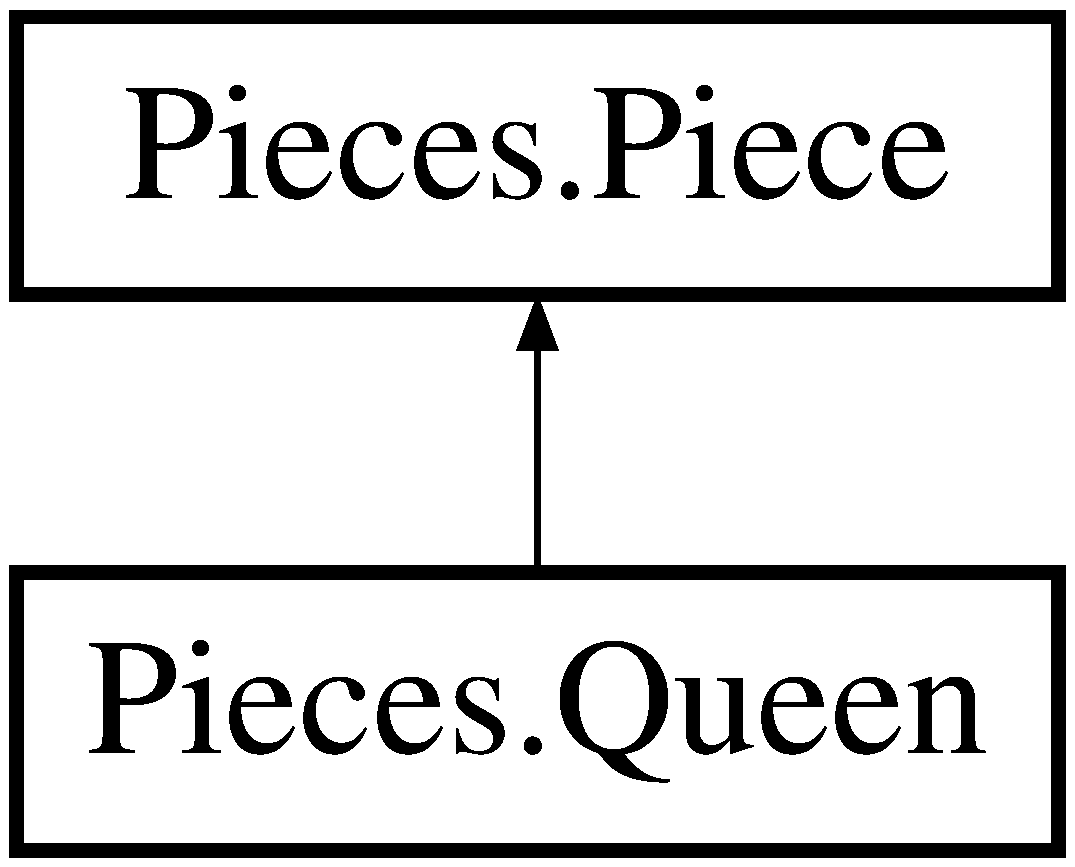
\includegraphics[height=2.000000cm]{classPieces_1_1Queen}
\end{center}
\end{figure}
\subsection*{Public Member Functions}
\begin{DoxyCompactItemize}
\item 
\hyperlink{classPieces_1_1Queen_ac0848f1b0969ccd73bf865f64f16a7aa}{Queen} (\hyperlink{classPieces_1_1Board}{Board} board, \hyperlink{classPieces_1_1Location}{Location} location, boolean owner)
\item 
boolean \hyperlink{classPieces_1_1Queen_a13541bde1a9418c2e53329d267df8f14}{valid\-Move} (int des\-\_\-x, int des\-\_\-y)
\end{DoxyCompactItemize}


\subsection{Detailed Description}
Created by yutong on 9/7/16. 

\subsection{Constructor \& Destructor Documentation}
\hypertarget{classPieces_1_1Queen_ac0848f1b0969ccd73bf865f64f16a7aa}{\index{Pieces\-::\-Queen@{Pieces\-::\-Queen}!Queen@{Queen}}
\index{Queen@{Queen}!Pieces::Queen@{Pieces\-::\-Queen}}
\subsubsection[{Queen}]{\setlength{\rightskip}{0pt plus 5cm}Pieces.\-Queen.\-Queen (
\begin{DoxyParamCaption}
\item[{{\bf Board}}]{board, }
\item[{{\bf Location}}]{location, }
\item[{boolean}]{owner}
\end{DoxyParamCaption}
)\hspace{0.3cm}{\ttfamily [inline]}}}\label{classPieces_1_1Queen_ac0848f1b0969ccd73bf865f64f16a7aa}
constructor for queen 
\begin{DoxyParams}{Parameters}
{\em board} & game board \\
\hline
{\em location} & piece location \\
\hline
{\em owner} & piece owner \\
\hline
\end{DoxyParams}


\subsection{Member Function Documentation}
\hypertarget{classPieces_1_1Queen_a13541bde1a9418c2e53329d267df8f14}{\index{Pieces\-::\-Queen@{Pieces\-::\-Queen}!valid\-Move@{valid\-Move}}
\index{valid\-Move@{valid\-Move}!Pieces::Queen@{Pieces\-::\-Queen}}
\subsubsection[{valid\-Move}]{\setlength{\rightskip}{0pt plus 5cm}boolean Pieces.\-Queen.\-valid\-Move (
\begin{DoxyParamCaption}
\item[{int}]{des\-\_\-x, }
\item[{int}]{des\-\_\-y}
\end{DoxyParamCaption}
)\hspace{0.3cm}{\ttfamily [inline]}, {\ttfamily [virtual]}}}\label{classPieces_1_1Queen_a13541bde1a9418c2e53329d267df8f14}

\begin{DoxyParams}{Parameters}
{\em des\-\_\-x} & coordinate x of destination tile \\
\hline
{\em des\-\_\-y} & coordinate y of destination tile \\
\hline
\end{DoxyParams}
\begin{DoxyReturn}{Returns}
return true if it's a valid queen move and no piece is blocking it, false o/w 
\end{DoxyReturn}


Implements \hyperlink{classPieces_1_1Piece}{Pieces.\-Piece}.



The documentation for this class was generated from the following file\-:\begin{DoxyCompactItemize}
\item 
src/\-Pieces/Queen.\-java\end{DoxyCompactItemize}

\hypertarget{classTests_1_1QueenTest}{\section{Tests.\-Queen\-Test Class Reference}
\label{classTests_1_1QueenTest}\index{Tests.\-Queen\-Test@{Tests.\-Queen\-Test}}
}
\subsection*{Public Member Functions}
\begin{DoxyCompactItemize}
\item 
\hypertarget{classTests_1_1QueenTest_a99dddb3dbcd30fc56fdf0fd35c8a9e55}{void {\bfseries test} ()}\label{classTests_1_1QueenTest_a99dddb3dbcd30fc56fdf0fd35c8a9e55}

\item 
\hypertarget{classTests_1_1QueenTest_a0119deab223fc6feed8df0fa0e11598a}{void {\bfseries is\-Valid} ()}\label{classTests_1_1QueenTest_a0119deab223fc6feed8df0fa0e11598a}

\end{DoxyCompactItemize}


\subsection{Detailed Description}
Created by yutong on 9/7/16. 

The documentation for this class was generated from the following file\-:\begin{DoxyCompactItemize}
\item 
src/\-Tests/Queen\-Test.\-java\end{DoxyCompactItemize}

\hypertarget{classPieces_1_1Rook}{\section{Pieces.\-Rook Class Reference}
\label{classPieces_1_1Rook}\index{Pieces.\-Rook@{Pieces.\-Rook}}
}
Inheritance diagram for Pieces.\-Rook\-:\begin{figure}[H]
\begin{center}
\leavevmode
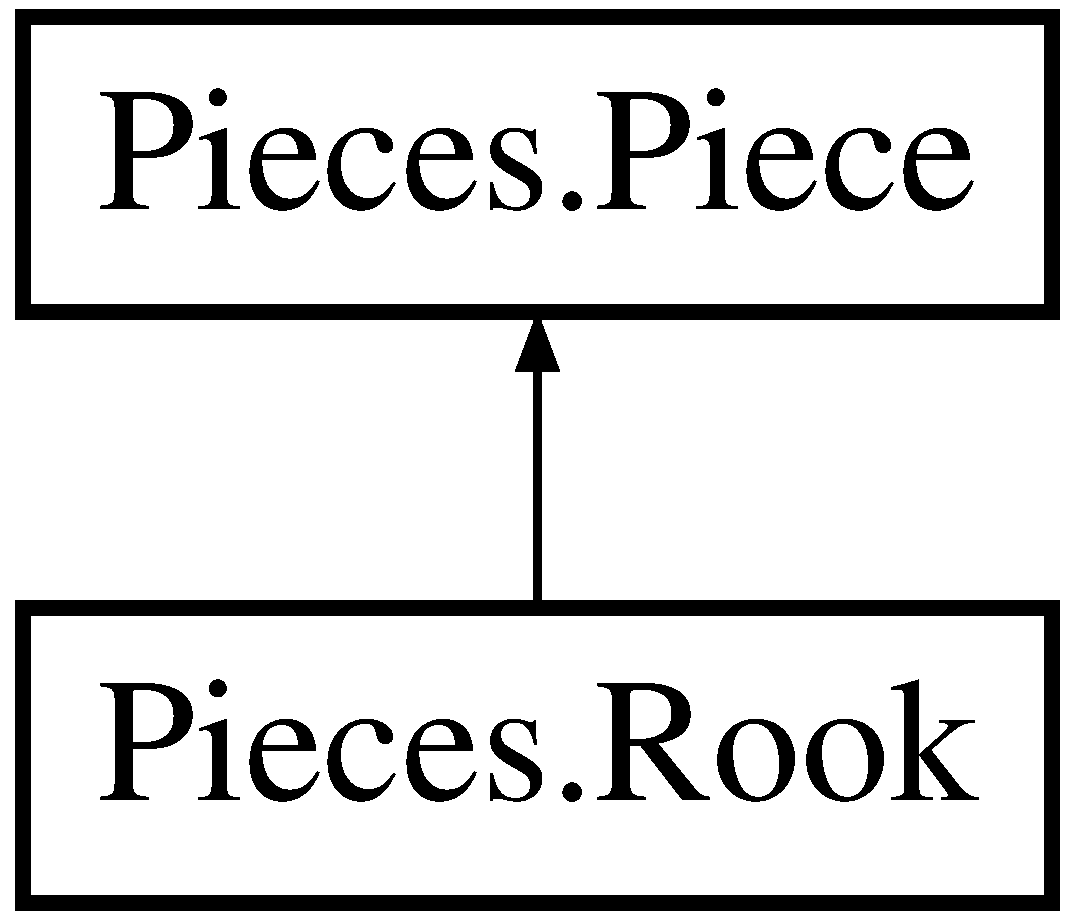
\includegraphics[height=2.000000cm]{classPieces_1_1Rook}
\end{center}
\end{figure}
\subsection*{Public Member Functions}
\begin{DoxyCompactItemize}
\item 
\hyperlink{classPieces_1_1Rook_ae47873d63e96c7311483438496ac0c84}{Rook} (\hyperlink{classPieces_1_1Board}{Board} board, \hyperlink{classPieces_1_1Location}{Location} location, boolean owner)
\item 
boolean \hyperlink{classPieces_1_1Rook_a4a5ff8db747f19ce44ad2d3b53559c57}{valid\-Move} (int des\-\_\-x, int des\-\_\-y)
\end{DoxyCompactItemize}


\subsection{Detailed Description}
Created by yutong on 9/7/16. 

\subsection{Constructor \& Destructor Documentation}
\hypertarget{classPieces_1_1Rook_ae47873d63e96c7311483438496ac0c84}{\index{Pieces\-::\-Rook@{Pieces\-::\-Rook}!Rook@{Rook}}
\index{Rook@{Rook}!Pieces::Rook@{Pieces\-::\-Rook}}
\subsubsection[{Rook}]{\setlength{\rightskip}{0pt plus 5cm}Pieces.\-Rook.\-Rook (
\begin{DoxyParamCaption}
\item[{{\bf Board}}]{board, }
\item[{{\bf Location}}]{location, }
\item[{boolean}]{owner}
\end{DoxyParamCaption}
)\hspace{0.3cm}{\ttfamily [inline]}}}\label{classPieces_1_1Rook_ae47873d63e96c7311483438496ac0c84}
constructor for rook 
\begin{DoxyParams}{Parameters}
{\em board} & game board \\
\hline
{\em location} & piece location \\
\hline
{\em owner} & piece owner \\
\hline
\end{DoxyParams}


\subsection{Member Function Documentation}
\hypertarget{classPieces_1_1Rook_a4a5ff8db747f19ce44ad2d3b53559c57}{\index{Pieces\-::\-Rook@{Pieces\-::\-Rook}!valid\-Move@{valid\-Move}}
\index{valid\-Move@{valid\-Move}!Pieces::Rook@{Pieces\-::\-Rook}}
\subsubsection[{valid\-Move}]{\setlength{\rightskip}{0pt plus 5cm}boolean Pieces.\-Rook.\-valid\-Move (
\begin{DoxyParamCaption}
\item[{int}]{des\-\_\-x, }
\item[{int}]{des\-\_\-y}
\end{DoxyParamCaption}
)\hspace{0.3cm}{\ttfamily [inline]}, {\ttfamily [virtual]}}}\label{classPieces_1_1Rook_a4a5ff8db747f19ce44ad2d3b53559c57}

\begin{DoxyParams}{Parameters}
{\em des\-\_\-x} & coordinate x of destination tile \\
\hline
{\em des\-\_\-y} & coordinate y of destination tile \\
\hline
\end{DoxyParams}
\begin{DoxyReturn}{Returns}
return true if it's a valid rook move and no piece is blocking it, false o/w 
\end{DoxyReturn}


Implements \hyperlink{classPieces_1_1Piece}{Pieces.\-Piece}.



The documentation for this class was generated from the following file\-:\begin{DoxyCompactItemize}
\item 
src/\-Pieces/Rook.\-java\end{DoxyCompactItemize}

\hypertarget{classTests_1_1RookTest}{\section{Tests.\-Rook\-Test Class Reference}
\label{classTests_1_1RookTest}\index{Tests.\-Rook\-Test@{Tests.\-Rook\-Test}}
}
\subsection*{Public Member Functions}
\begin{DoxyCompactItemize}
\item 
\hypertarget{classTests_1_1RookTest_a8f59ba2ae46379636878d9c3b66aeb1e}{void {\bfseries test} ()}\label{classTests_1_1RookTest_a8f59ba2ae46379636878d9c3b66aeb1e}

\item 
\hypertarget{classTests_1_1RookTest_a63f02c95ad7e4fed50f3a647bbd6f710}{void {\bfseries is\-Valid} ()}\label{classTests_1_1RookTest_a63f02c95ad7e4fed50f3a647bbd6f710}

\end{DoxyCompactItemize}


\subsection{Detailed Description}
Created by yutong on 9/7/16. 

The documentation for this class was generated from the following file\-:\begin{DoxyCompactItemize}
\item 
src/\-Tests/Rook\-Test.\-java\end{DoxyCompactItemize}

\hypertarget{classPieces_1_1SpecialBishop}{\section{Pieces.\-Special\-Bishop Class Reference}
\label{classPieces_1_1SpecialBishop}\index{Pieces.\-Special\-Bishop@{Pieces.\-Special\-Bishop}}
}
Inheritance diagram for Pieces.\-Special\-Bishop\-:\begin{figure}[H]
\begin{center}
\leavevmode
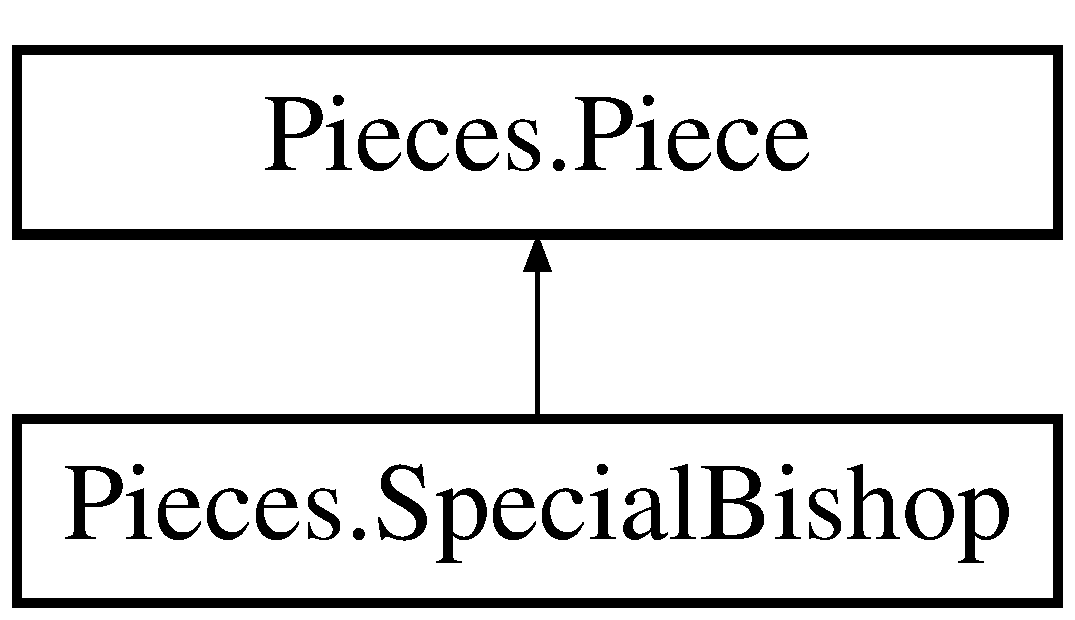
\includegraphics[height=2.000000cm]{classPieces_1_1SpecialBishop}
\end{center}
\end{figure}
\subsection*{Public Member Functions}
\begin{DoxyCompactItemize}
\item 
\hyperlink{classPieces_1_1SpecialBishop_a8a34e91f32032f3e54bffbe8a701352d}{Special\-Bishop} (\hyperlink{classPieces_1_1Board}{Board} board, \hyperlink{classPieces_1_1Location}{Location} location, boolean owner)
\item 
boolean \hyperlink{classPieces_1_1SpecialBishop_a478a8c0332931da570772e4abe5405fd}{valid\-Move} (int des\-\_\-x, int des\-\_\-y)
\end{DoxyCompactItemize}


\subsection{Detailed Description}
Created by yutong on 9/14/16. 

\subsection{Constructor \& Destructor Documentation}
\hypertarget{classPieces_1_1SpecialBishop_a8a34e91f32032f3e54bffbe8a701352d}{\index{Pieces\-::\-Special\-Bishop@{Pieces\-::\-Special\-Bishop}!Special\-Bishop@{Special\-Bishop}}
\index{Special\-Bishop@{Special\-Bishop}!Pieces::SpecialBishop@{Pieces\-::\-Special\-Bishop}}
\subsubsection[{Special\-Bishop}]{\setlength{\rightskip}{0pt plus 5cm}Pieces.\-Special\-Bishop.\-Special\-Bishop (
\begin{DoxyParamCaption}
\item[{{\bf Board}}]{board, }
\item[{{\bf Location}}]{location, }
\item[{boolean}]{owner}
\end{DoxyParamCaption}
)\hspace{0.3cm}{\ttfamily [inline]}}}\label{classPieces_1_1SpecialBishop_a8a34e91f32032f3e54bffbe8a701352d}
constructor for special bishop 
\begin{DoxyParams}{Parameters}
{\em board} & game board \\
\hline
{\em location} & piece location \\
\hline
{\em owner} & piece owner \\
\hline
\end{DoxyParams}


\subsection{Member Function Documentation}
\hypertarget{classPieces_1_1SpecialBishop_a478a8c0332931da570772e4abe5405fd}{\index{Pieces\-::\-Special\-Bishop@{Pieces\-::\-Special\-Bishop}!valid\-Move@{valid\-Move}}
\index{valid\-Move@{valid\-Move}!Pieces::SpecialBishop@{Pieces\-::\-Special\-Bishop}}
\subsubsection[{valid\-Move}]{\setlength{\rightskip}{0pt plus 5cm}boolean Pieces.\-Special\-Bishop.\-valid\-Move (
\begin{DoxyParamCaption}
\item[{int}]{des\-\_\-x, }
\item[{int}]{des\-\_\-y}
\end{DoxyParamCaption}
)\hspace{0.3cm}{\ttfamily [inline]}, {\ttfamily [virtual]}}}\label{classPieces_1_1SpecialBishop_a478a8c0332931da570772e4abe5405fd}

\begin{DoxyParams}{Parameters}
{\em des\-\_\-x} & coordinate x of destination tile \\
\hline
{\em des\-\_\-y} & coordinate y of destination tile \\
\hline
\end{DoxyParams}
\begin{DoxyReturn}{Returns}
moves like a bishop except no piece can block it 
\end{DoxyReturn}


Implements \hyperlink{classPieces_1_1Piece}{Pieces.\-Piece}.



The documentation for this class was generated from the following file\-:\begin{DoxyCompactItemize}
\item 
src/\-Pieces/Special\-Bishop.\-java\end{DoxyCompactItemize}

\hypertarget{classPieces_1_1SpecialRook}{\section{Pieces.\-Special\-Rook Class Reference}
\label{classPieces_1_1SpecialRook}\index{Pieces.\-Special\-Rook@{Pieces.\-Special\-Rook}}
}
Inheritance diagram for Pieces.\-Special\-Rook\-:\begin{figure}[H]
\begin{center}
\leavevmode
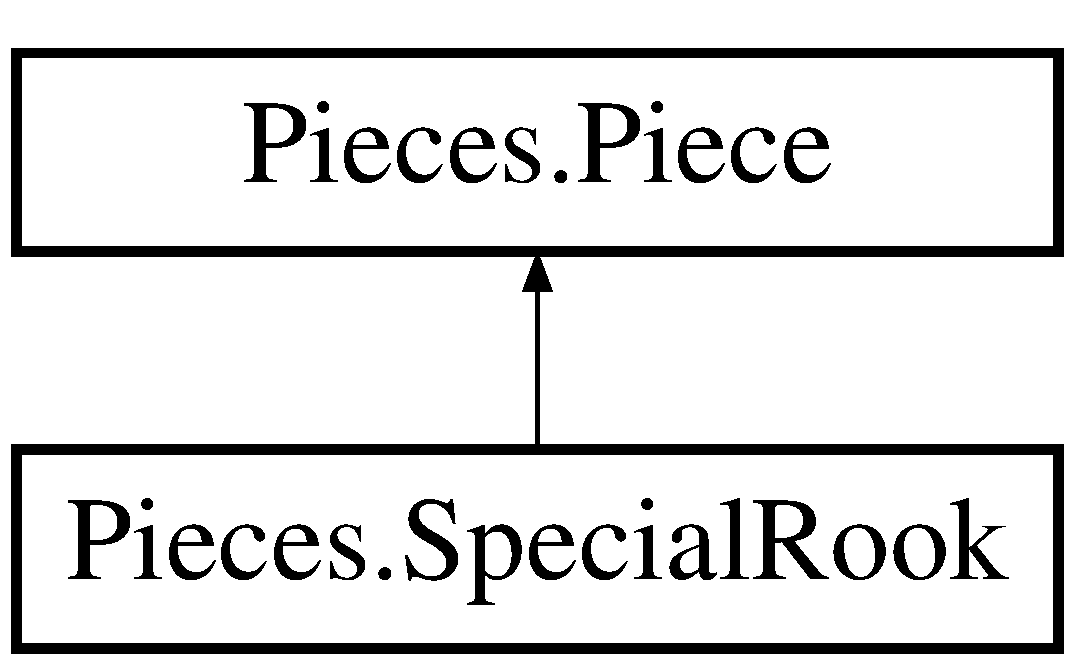
\includegraphics[height=2.000000cm]{classPieces_1_1SpecialRook}
\end{center}
\end{figure}
\subsection*{Public Member Functions}
\begin{DoxyCompactItemize}
\item 
\hyperlink{classPieces_1_1SpecialRook_a9aa8bc9c984f1abb2b625ef5f437e843}{Special\-Rook} (\hyperlink{classPieces_1_1Board}{Board} board, \hyperlink{classPieces_1_1Location}{Location} location, boolean owner)
\item 
boolean \hyperlink{classPieces_1_1SpecialRook_a605a972351e3bc6221a4071112aa179d}{valid\-Move} (int des\-\_\-x, int des\-\_\-y)
\end{DoxyCompactItemize}


\subsection{Detailed Description}
Created by yutong on 9/14/16. 

\subsection{Constructor \& Destructor Documentation}
\hypertarget{classPieces_1_1SpecialRook_a9aa8bc9c984f1abb2b625ef5f437e843}{\index{Pieces\-::\-Special\-Rook@{Pieces\-::\-Special\-Rook}!Special\-Rook@{Special\-Rook}}
\index{Special\-Rook@{Special\-Rook}!Pieces::SpecialRook@{Pieces\-::\-Special\-Rook}}
\subsubsection[{Special\-Rook}]{\setlength{\rightskip}{0pt plus 5cm}Pieces.\-Special\-Rook.\-Special\-Rook (
\begin{DoxyParamCaption}
\item[{{\bf Board}}]{board, }
\item[{{\bf Location}}]{location, }
\item[{boolean}]{owner}
\end{DoxyParamCaption}
)\hspace{0.3cm}{\ttfamily [inline]}}}\label{classPieces_1_1SpecialRook_a9aa8bc9c984f1abb2b625ef5f437e843}
constructor for special rook 
\begin{DoxyParams}{Parameters}
{\em board} & game board \\
\hline
{\em location} & piece location \\
\hline
{\em owner} & piece owner \\
\hline
\end{DoxyParams}


\subsection{Member Function Documentation}
\hypertarget{classPieces_1_1SpecialRook_a605a972351e3bc6221a4071112aa179d}{\index{Pieces\-::\-Special\-Rook@{Pieces\-::\-Special\-Rook}!valid\-Move@{valid\-Move}}
\index{valid\-Move@{valid\-Move}!Pieces::SpecialRook@{Pieces\-::\-Special\-Rook}}
\subsubsection[{valid\-Move}]{\setlength{\rightskip}{0pt plus 5cm}boolean Pieces.\-Special\-Rook.\-valid\-Move (
\begin{DoxyParamCaption}
\item[{int}]{des\-\_\-x, }
\item[{int}]{des\-\_\-y}
\end{DoxyParamCaption}
)\hspace{0.3cm}{\ttfamily [inline]}, {\ttfamily [virtual]}}}\label{classPieces_1_1SpecialRook_a605a972351e3bc6221a4071112aa179d}

\begin{DoxyParams}{Parameters}
{\em des\-\_\-x} & coordinate x of destination tile \\
\hline
{\em des\-\_\-y} & coordinate y of destination tile \\
\hline
\end{DoxyParams}
\begin{DoxyReturn}{Returns}
moves like a rook except no piece can block it 
\end{DoxyReturn}


Implements \hyperlink{classPieces_1_1Piece}{Pieces.\-Piece}.



The documentation for this class was generated from the following file\-:\begin{DoxyCompactItemize}
\item 
src/\-Pieces/Special\-Rook.\-java\end{DoxyCompactItemize}

\addcontentsline{toc}{part}{Index}
\printindex
\end{document}
